\documentclass[12pt,spanish,Letterpaper,openany]{book}
\usepackage{lmodern}
\usepackage{setspace}
\setstretch{0.85}
\usepackage{amssymb,amsmath}
\usepackage{ifxetex,ifluatex}
\usepackage{fixltx2e} % provides \textsubscript
\ifnum 0\ifxetex 1\fi\ifluatex 1\fi=0 % if pdftex
  \usepackage[T1]{fontenc}
  \usepackage[utf8]{inputenc}
\else % if luatex or xelatex
  \ifxetex
    \usepackage{mathspec}
  \else
    \usepackage{fontspec}
  \fi
  \defaultfontfeatures{Ligatures=TeX,Scale=MatchLowercase}
    \setmainfont[Scale=1.0, HyphenChar=None]{Corbel}
    \setsansfont[]{Corbel}
    \setmonofont[Mapping=tex-ansi]{Corbel}
\fi

\makeatletter
\renewcommand\mainmatter{\clearpage\@mainmattertrue\pagenumbering{arabic}}
\renewcommand\frontmatter{\clearpage\@mainmatterfalse\pagenumbering{arabic}}
\renewcommand\backmatter{\clearpage\@mainmatterfalse}
\makeatother

%\usepackage{etoolbox}
%\makeatletter
%\patchcmd{\@smemmain}{\cleardoublepage}{\clearpage}{}{}
%\patchcmd{\@smemmain}{\cleardoublepage}{\clearpage}{}{}
%\patchcmd{\@smemfront}{\cleardoublepage}{\clearpage}{}{}
%\patchcmd{\@smemfront}{\cleardoublepage}{\clearpage}{}{}
%\makeatother

\setlength{\parindent}{0em}

\usepackage{graphicx}
\usepackage{booktabs}
\usepackage{multicol}
\usepackage{doc}
\usepackage{float}
\usepackage{tcolorbox} 
\usepackage{lipsum}
\usepackage{tikz}
\usepackage{nonfloat}

\usepackage{pdfpages}

\usepackage[
contents={},
opacity=1,
scale=1.5,
color=blue!90
]{background}
\usepackage{lipsum}
\usepackage{ifthen}

\usepackage{xcolor}
\usepackage[pagestyles]{titlesec}

\renewpagestyle{plain}[\normalsize\sffamily\bfseries\slshape]{
  \setfoot{}{\color{white}{\thepage}}{}}

\newpagestyle{myps}[\normalsize\sffamily\bfseries\slshape]{
  \setfoot{}{\color{white}{\thepage}}{}}
  
\pagestyle{myps}


\usepackage{framed}
\definecolor{colorlinetitle}{HTML}{a87e00}%{a87e00}%
\definecolor{textlinetitle}{HTML}{061769}%{061769}%{061769}%
\definecolor{fondo}{HTML}{041d57}%
\definecolor{newfondo}{HTML}{3d0718}%
\colorlet{shadecolor}{fondo!81!}


% use upquote if available, for straight quotes in verbatim environments
\IfFileExists{upquote.sty}{\usepackage{upquote}}{}
% use microtype if available
\IfFileExists{microtype.sty}{%
\usepackage{microtype}
\UseMicrotypeSet[protrusion]{basicmath} % disable protrusion for tt fonts
}{}
\usepackage[inner=12.7mm,outer=12.7mm,top=13mm,bottom=21.0mm]{geometry}
\usepackage{hyperref}
\hypersetup{unicode=true,
            pdftitle={Revista digital de la unidad de prácticas de ingeniería y EPS},
            pdfauthor={Unidad de Ejercicio Profesional Supervisado},
            pdfborder={0 0 0},
            breaklinks=true}
\urlstyle{same}  % don't use monospace font for urls
\ifnum 0\ifxetex 1\fi\ifluatex 1\fi=0 % if pdftex
  \usepackage[shorthands=off,main=spanish]{babel}
\else
  \usepackage{polyglossia}
  \setmainlanguage[]{spanish}
\fi
\usepackage{natbib}
\bibliographystyle{apalike}
\usepackage{longtable,booktabs}
\IfFileExists{parskip.sty}{%
\usepackage{parskip}
}{% else
\setlength{\parindent}{0pt}
\setlength{\parskip}{6pt plus 2pt minus 1pt}
}
\setlength{\emergencystretch}{3em}  % prevent overfull lines
\providecommand{\tightlist}{%
  \setlength{\itemsep}{0pt}\setlength{\parskip}{0pt}}
\setcounter{secnumdepth}{5}
% Redefines (sub)paragraphs to behave more like sections
\ifx\paragraph\undefined\else
\let\oldparagraph\paragraph
\renewcommand{\paragraph}[1]{\oldparagraph{#1}\mbox{}}
\fi
\ifx\subparagraph\undefined\else
\let\oldsubparagraph\subparagraph
\renewcommand{\subparagraph}[1]{\oldsubparagraph{#1}\mbox{}}
\fi

%%% Use protect on footnotes to avoid problems with footnotes in titles
\let\rmarkdownfootnote\footnote%
\def\footnote{\protect\rmarkdownfootnote}


  \title{Revista digital de la unidad de prácticas de ingeniería y EPS}
    \author{Unidad de Ejercicio Profesional Supervisado}
      \date{2022-11-04}

% no title page
\AtBeginDocument{\let\maketitle\relax}

\usepackage{caption}[=v1]


\usepackage{booktabs}
\usepackage{longtable}

\usepackage{indentfirst}
\setlength{\parindent}{1em}
\usepackage{enumitem}
\setlist[itemize]{labelindent = \parindent, leftmargin=*}

%\usepackage{framed,color}
%\definecolor{shadecolor}{RGB}{248,248,248}

\renewcommand{\textfraction}{0.05}
\renewcommand{\topfraction}{0.8}
\renewcommand{\bottomfraction}{0.8}
\renewcommand{\floatpagefraction}{0.75}

\renewcommand{\chaptername}{Artículo}
\addto\captionsspanish{\renewcommand{\chaptername}{Artículo}}
\addto\captionsspanish{\renewcommand{\contentsname}{Índice general}}


\frenchspacing
\tolerance=5000
\multicoltolerance=3000 

\raggedbottom
\raggedcolumns

\setlength{\columnsep}{1em}
%We want a rule between columns.
%\setlength\columnseprule{.4pt}

%Tambien queremos asegurarnos de que un nuevo entorno multicols 
%encuentre suficiente espacio en la parte inferior de la pagina.
\setlength\premulticols{6\baselineskip}

%Al equilibrar columnas, ignoramos las soluciones que son 
%demasiado malas. Ademas, si la ultima columna es demasiado mala, 
%la tipeamos sin estirar.
\setcounter{columnbadness}{7000}
\setcounter{finalcolumnbadness}{7000}

\newcommand{\prefacetitlecommand}%
{\titleformat{\chapter}[display]%
{\bfseries\large\color{colorlinetitle}}%
{\relax}%
{0ex}%
{{\titlerule[1.2pt]}\filcenter\color{textlinetitle}}[\color{colorlinetitle}\vspace{0.5ex}{\titlerule[1.2pt]}]%
}


\newcommand{\articletitlecommand}%
{\titleformat{\chapter}[display]%
{\bfseries\Large\centering\color{white}}%
{\relax}%
{0ex}%
{{\titlerule[1.2pt]}\filcenter\color{textlinetitle}}[\color{white}\vspace{0.5ex}{\titlerule[1.2pt]}]%
}



\newcommand{\sectionCenter}%
{\titleformat{\section}[block]%
{\bfseries\large\color{textlinetitle}\filcenter}%
{\relax}%
{0ex}%
{\empty}%
}


\newcommand{\sectionRight}%
{\titleformat{\section}[block]%
{\bfseries\large\color{textlinetitle}}%
{\relax}%
{0ex}%
{\empty}%
}


\newcommand{\subsectionRight}%
{\titleformat{\subsection}[block]%
{\bfseries\normalsize\color{textlinetitle}}%
{\relax}%
{0ex}%
{\empty}%
}

\usepackage{titletoc}
\titlecontents{chapter}[3em]
{\vspace{5mm}}
{\normalsize\contentslabel[\color{textlinetitle}\thecontentslabel]{2em}\color{black}\itshape\normalsize}
{\color{black}\itshape\normalsize}
{\color{colorlinetitle}\titlerule*[.3pc]{.}\color{black}\contentspage}

\newcommand{\tcolorboxcommand}{\begin{tcolorbox}[sharp corners=uphill, colback=newfondo, colframe=newfondo, arc=6mm, boxrule=0mm, boxsep=0mm]}

\newcommand{\photocommand}[2]{%
\fcolorbox[HTML]{DCEEA7}{DCEEA7}{%
\begin{minipage}{95.19mm}%
	\hspace{1mm}%
	\begin{minipage}{22.49mm}%
		\vspace{1mm}%
		\includegraphics[width=22.49mm, height=31.96mm]{#1}%
		\vspace{1mm}%
	\end{minipage}%
	\hspace{2.4mm}%
	\begin{minipage}{68.80mm}%
		#2
	\end{minipage}%
	\hspace{0.5mm}%
\end{minipage}%
}%
}

\definecolor{fondobiography}{HTML}{DCEEA7}

\NewDocumentEnvironment{photobiography}{m O{}}%
{%
\begin{tcolorbox}[colback=fondobiography, colframe=fondobiography, width=97.19mm, boxsep=-2mm, arc=0mm]
\begin{minipage}{95.19mm}%
	%\hspace{1mm}%
	\begin{minipage}{22.49mm}%
		\vspace{2mm}%
		\includegraphics[width=22.49mm, height=31.96mm]{#1}%
		\vspace{2mm}%
	\end{minipage}%
	\hspace{2.4mm}%
	\begin{minipage}{68.80mm}%
	#2%
}%
{%
	\end{minipage}%
	%\hspace{0.5mm}%
\end{minipage}%
\end{tcolorbox}
}


\newcommand{\spacetext}{\vspace{8.1mm}}
\newcommand{\minimalspacetext}{\vspace{1mm}}
\newcommand{\spaceelevenmilis}{\vspace{11mm}}
\newcommand{\spacetenmilis}{\vspace{10mm}}
\newcommand{\spaceninemilis}{\vspace{9mm}}
\newcommand{\spaceeightmilis}{\vspace{8mm}}
\newcommand{\spacesevenmilis}{\vspace{7mm}}
\newcommand{\spacesixmilis}{\vspace{6mm}}
\newcommand{\spacefivemilis}{\vspace{5mm}}
\newcommand{\spacefourmilis}{\vspace{4mm}}
\newcommand{\spacethreemilis}{\vspace{3mm}}
\newcommand{\spacetwomilis}{\vspace{2mm}}
\newcommand{\spaceinitialeditorialcontenido}{\vspace{8.1mm}}
\newcommand{\spaceoneminus}{\vspace{-1mm}}
\newcommand{\spacetwominus}{\vspace{-2mm}}
\newcommand{\spacefourminus}{\vspace{-4mm}}
\newcommand{\hideFromPandoc}[1]{#1}
\hideFromPandoc{ \let\Begin\begin \let\End\end }
\newcommand{\minipagepartone}{\begin{minipage}[c]{3cm}}
\newcommand{\minipagetwocolumn}{\noindent\begin{minipage}[c]{\columnwidth}}
\newcommand{\minipageparttwo}{\end{minipage}\begin{minipage}[c]{12cm}}
\newcommand{\minipageparttwochapter}{\end{minipage}\begin{minipage}[c]{15cm}}
\newcommand{\minipageendpart}{\end{minipage}}
\newcommand{\firstparteditorial}{\begin{longtable}[]{@{}ll@{}}\endhead\begin{minipage}[t]{0.47\columnwidth}\raggedright}
\newcommand{\firstparttwoeditorial}{\begin{longtable}[l]{@{}ll@{}}\endhead\begin{minipage}[t]{0.47\columnwidth}\raggedright}
\newcommand{\midleparteditorial}{\end{minipage} & \begin{minipage}[t]{0.47\columnwidth}\raggedright}
\newcommand{\lastparteditorial}{\end{minipage}\end{longtable}}

\newcommand{\HRule}{\begin{center}\rule{0.5\linewidth}{0.2mm}\end{center}}

\begin{document}
\maketitle

% \pagestyle{plain}

\includepdf{images/cover.pdf}

\AddEverypageHook{%
\ifthenelse{\value{page}<40}%
{\ifthenelse{\isodd{\value{page}}}%
  	{\backgroundsetup{scale=1, color=black, opacity=0, angle=0, contents={
\includegraphics[width=\paperwidth,height=\paperheight]{latex/background_numberimpar.pdf}}}}%
  	{\backgroundsetup{scale=1, color=black, opacity=0, angle=0, contents={
\includegraphics[width=\paperwidth,height=\paperheight]{latex/background_numberpar.pdf}}}}%
}{}%
\BgMaterial}

%%%%%%{
%%%%%%\setcounter{tocdepth}{0}
%%%\tableofcontents
%%%}
%%%%%%%%%%%%\listoffigures
%%%
\prefacetitlecommand

\titlespacing*{\chapter} {0pt}{0pt}{0pt}

\titleformat{\chapter}[display]
{\normalfont\color{textlinetitle} \bfseries}
{\empty}
{0pt}
{\filcenter\Huge}

\spacetenmilis
\spacetenmilis
\spacetenmilis
\spacetenmilis

\hypertarget{editorial}{%
\chapter*{Editorial}\label{editorial}}
\addcontentsline{toc}{chapter}{Editorial}

\begin{center}
\includegraphics[width=1\linewidth]{images/editorial} \end{center}

\titleformat{\chapter}[display]
{\normalfont\color{textlinetitle} \bfseries}
{\empty}
{0pt}
{\filcenter\Huge}

\titleformat{\chapter}[display]
{\normalfont\color{textlinetitle} \bfseries}
{\empty}
{0pt}
{\filcenter\Huge}

\hypertarget{nomina}{%
\chapter*{Nómina de Junta Directiva}\label{nomina}}
\addcontentsline{toc}{chapter}{Nómina de Junta Directiva}

\spacetenmilis
\spacetenmilis
\spacetenmilis

\begin{center}
\includegraphics[width=0.4\linewidth]{images/logo} \end{center}

\spacethreemilis
\spacethreemilis
\spacethreemilis

\begin{longtable}[]{@{}cc@{}}
\toprule
\endhead
DECANA & INGA. AURELIA ANABELA CORDOVA ESTRADA\tabularnewline
VOCAL I & ING. JOSÉ FRANCISCO GÓMEZ RIVERA\tabularnewline
VOCAL II & ING. MARIO RENATO ESCOBEDO MARTINEZ\tabularnewline
VOCAL III & ING. JOSÉ MILTON DE LEÓN BRAN\tabularnewline
VOCAL IV & BR. KEVIN VLADIMIR CRUZ LORENTE\tabularnewline
VOCAL V & BR. FERNANDO JOSÉ PAZ GONZÁLEZ\tabularnewline
SECRETARIO & ING. HUGO HUMBERTO RIVERA PÉREZ\tabularnewline
\bottomrule
\end{longtable}

\titleformat{\chapter}[display]
{\normalfont\color{textlinetitle} \bfseries}
{\empty}
{0pt}
{\filcenter\Huge}

\titleformat{\chapter}[display]
{\normalfont\color{textlinetitle} \bfseries}
{\empty}
{0pt}
{\filcenter\Huge}

\spacetenmilis
\spacetenmilis
\spacetenmilis
\spacetenmilis
\spacetenmilis
\spacetenmilis
\spacetenmilis
\spacetenmilis
\spacetenmilis
\spacetenmilis
\spacetenmilis
\spacetenmilis

\hypertarget{directorio}{%
\chapter*{Directorio}\label{directorio}}
\addcontentsline{toc}{chapter}{Directorio}

\spacethreemilis
\spacethreemilis

\begin {multicols}{2}

\hypertarget{director}{%
\section*{Director de la revista}\label{director}}
\addcontentsline{toc}{section}{Director de la revista}

\textbf{Ingeniero Oscar Argueta Hernández}

Dirección de Prácticas de Ingeniería y EPS

\hypertarget{editor}{%
\section*{Editor en jefe}\label{editor}}
\addcontentsline{toc}{section}{Editor en jefe}

\textbf{Ingeniera Floriza Avila Pesquera de Medinilla}

Coordinadora del Área de Tecnología

Unidad de Prácticas de Ingeniería

\hypertarget{coeditores}{%
\section*{Coeditores}\label{coeditores}}
\addcontentsline{toc}{section}{Coeditores}

\textbf{Ingeniero Juan Merck Cos}

Asesor Supervisor del Área de Ingeniería Civil

Unidad de Prácticas de Ingeniería

\spacethreemilis

\textbf{Ingeniero Silvio José Rodríguez Serrano}

Asesor Supervisor del Área de Ingeniería Civil

Unidad de Prácticas de Ingeniería

\spacethreemilis

\textbf{Ingeniera Sigrid Alitza Calderón de De Léon}

Asesor Supervisor del Área de Ingeniería Industrial

y Mecánica Industrial Unidad de Prácticas

de Ingeniería

\spacethreemilis

\hypertarget{consejoeditorial}{%
\section*{Consejo Editorial}\label{consejoeditorial}}
\addcontentsline{toc}{section}{Consejo Editorial}

\textbf{Ingeniero Oscar Argueta Hernández}

Asesor Supervisor del Área de Ingeniería Civil

Unidad de Prácticas de Ingeniería

\spacethreemilis

\textbf{Ingeniera Floriza Avila Pesquera de Medinilla}

Asesor Supervisor del Área de Ingeniería de

Ciencias y Sistemas

Unidad de Prácticas de Ingeniería

\spacethreemilis

\textbf{Ingeniero Juan Merck Cos}

Asesor Supervisor del Área de Ingeniería Civil

Unidad de Prácticas de Ingeniería

\spacethreemilis

\textbf{Ingeniero Carlos Anibal Chicojay Coloma}

Asesor Supervisor del Área de Ingeniería Mecánica

Unidad de Prácticas de Ingeniería

\spacethreemilis

\textbf{Ingeniera Sigrid Alitza Calderón de De Léon}

Asesor Supervisor del Área de Ingeniería Industrial

y Mecánica Industrial

Unidad de Prácticas de Ingeniería

\spacethreemilis

\textbf{Ingeniera Norma Ileana Sarmiento de Serrano}

Asesor Supervisor del Área de Ingeniería Industrial

y Mecánica Industrial

Unidad de Prácticas de Ingeniería

\end {multicols}

\titleformat{\chapter}[display]
{\normalfont\color{textlinetitle} \bfseries}
{\empty}
{0pt}
{\filcenter\Huge}

\titleformat{\chapter}[display]
{\normalfont\color{textlinetitle} \bfseries}
{\empty}
{0pt}
{\filcenter\Huge}

\hypertarget{comiteeditorial}{%
\chapter*{Comité editorial}\label{comiteeditorial}}
\addcontentsline{toc}{chapter}{Comité editorial}

\spacethreemilis
\spacethreemilis

\textbf{Ingeniero Oscar Argueta Hernández}

Asesor Supervisor del Área de Ingeniería Civil

Unidad de Prácticas de Ingeniería

\spacethreemilis

\textbf{Ingeniera Floriza Avila Pesquera de Medinilla}

Asesor Supervisor del Área de Ingeniería de Ciencias y Sistemas

Unidad de Prácticas de Ingeniería

\spacethreemilis

\textbf{Ingeniero Juan Merck Cos}

Asesor Supervisor del Área de Ingeniería Civil

Unidad de Prácticas de Ingeniería

\spacethreemilis

\textbf{Ingeniero Carlos Anibal Chicojay Coloma}

Asesor Supervisor del Área de Ingeniería Mecánica Unidad de Prácticas de Ingeniería

\spacethreemilis

\textbf{Ingeniera Sigrid Alitza Calderón de De Léon}

Asesor Supervisor del Área de Ingeniería Industrial y Mecánica Industrial

Unidad de Prácticas de Ingeniería

\spacethreemilis

\textbf{Ingeniera Norma Ileana Sarmiento de Serrano}

Asesor Supervisor del Área de Ingeniería Industrial y Mecánica Industrial

Unidad de Prácticas de Ingeniería

\spacethreemilis

\textbf{Ingeniero Silvio José Rodríguez Serrano}

Asesor Supervisor del Área de Ingeniería Civil

Unidad de Prácticas de Ingeniería

\spacethreemilis

\textbf{Licenciada Aura Mayorga Salguero}

Revisión y estilo

\spacethreemilis

\textbf{Augusto German Mazariegos Salguero}

Redacción, diseño y diagramación

Epesista Ingeniería en Ciencias y Sistemas

\setcounter{tocdepth}{0}
\tableofcontents

\articletitlecommand

\titlespacing*{\chapter} {0pt}{-39pt}{0pt}

\hypertarget{Cristian}{%
\chapter{Negocio componible inteligente}\label{Cristian}}

\begin{center}
\includegraphics[width=1\linewidth]{images/cJuarez_image1} \end{center}

\begin {multicols}{2}

\hypertarget{resumen}{%
\section{Resumen}\label{resumen}}

Una empresa componible inteligente es aquella que puede adaptarse y reorganizarse fundamentalmente en función de una situación actual. A medida que las organizaciones aceleran la estrategia comercial para impulsar una transformación digital más rápida, deben también ser ágiles y tomar decisiones comerciales rápidas con base en los datos disponibles en ese momento. Para hacer esto con éxito las organizaciones deben permitir un mejor acceso a la información, y aumentarla con un mejor conocimiento; luego, tener la capacidad de responder rápidamente a las implicaciones de dicho conocimien-
to. Esto también incluirá una mayor autonomía y democratización en toda la organización, lo que permitirá que partes de las empresas reaccionen rápidamente en lugar de verse empantanadas por procesos ineficientes.

\hypertarget{abstract}{%
\section{Abstract}\label{abstract}}

A smart composable company is one that can fundamentally adapt and reorganize itself based on a current situation. As organizations accelerate digital business strategy to drive faster digital transformation, they must be agile and make quick business decisions informed by the data available at the time. To do this successfully, organizations must allow better access to information, augment that information with better knowledge, and can respond quickly to the implications of that knowledge. This will also include greater autonomy and democratization throughout the organization, allowing parts of companies to react quickly rather than be bogged down by inefficient processes.

\hypertarget{palabras-claves}{%
\section{Palabras claves}\label{palabras-claves}}

Tendencia, automatización, descubrimiento, blo-
ques, adaptación.

\hypertarget{introducciuxf3n}{%
\section{Introducción}\label{introducciuxf3n}}

Según Gartner, citado por Burke (2020), para el 2021, una de las tendencias será el negocio componible inteligente. En un ambiente donde los negocios requieren múltiples cambios para mantener las ventajas o para no quedar definitivamente fuera de juego, las organizaciones necesitan ser capaces de adaptarse dinámicamente sin dejar de proponer innovaciones que se puedan aolicar de manera ágil. Es en este escenario donde toman relevancia las soluciones empresariales componibles.
Los Chief Information Officer (CIO) de los sectores público y privado están utilizando empresas componibles para buscar una mayor ventaja en tiempos de disrupción.

Los Chief Information Officer (CIO) de los sectores público y privado están utilizando empresas componi-
bles para buscar una mayor ventaja en tiempos de disrupción.

\hypertarget{artuxedculo}{%
\section{Artículo}\label{artuxedculo}}

\textbf{¿Qué son las soluciones empresariales componi-
bles}

Desde el punto de vista de la arquitectura de TI, una solución empresarial componible se basa en el uso de las API (Application Programming Interface) para proporcionar soluciones de valor al negocio.

Desde un punto de vista menos técnico, de lo que se trataría es de componer soluciones completas que se conectarían entre ellas, y proporcionarían aplicaciones para resolver problemas de inicio a fin.

Un ejemplo del uso de soluciones componibles puede ser la automatización inteligente. En estos casos se utiliza, habitualmente, BPM (Business Process Management) en combinación con AI (Artificial Intelligent) y RPA (Robotic Process Automa-
tion) para solucionar diferentes problemáticas en una empresa.
En términos simples, la automatización inteligente es la combinación de dos tecnologías base: inteligencia artificial y automatización. Un ejemplo directo es el funcionamiento de los automóviles autónomos, donde cientos de sensores recopilan y entregan información de forma automática (RPA) y una computadora central toma decisiones rápidas y certeras de acuerdo con reglas predefinidas (AI).

Negocio componible significa crear una organización hecha de bloques de construcción intercambiables (Saran, 2020).

El negocio componible es una aceleración natural del negocio digital en el que se vive todos los días. Permite ofrecer la resistencia y agilidad que exigen estos tiempos interesantes (Plummer, s. f).

La pandemia puso en relieve las vulnerabilidades en los modelos de negocio que durante años se centraron en la eficiencia. Las organizaciones que alguna vez fueron eficientes de repente se volvieron frágiles en un momento en el que se necesitaba que fueran flexibles. Ahora las empresas que eran inteligentes pivotan a una configuración más modular, llegando a la creación de una empresa componible. Estas estaban preparadas para un tipo de futuro, pero ahora deben de planificar múltiples futuros.

Negocio componible significa crear una organiza-
ción hecha de bloques de construcción intercambia-
bles. La configuración modular permite que una empresa se reorganice y reoriente según sea necesario en función de factores externos (o internos) como un cambio en los valores del cliente o un cambio repentino en la cadena de suministro o en los materiales.

Las organizaciones deben seguir los cuatro principios de modularidad empresarial: componible, autónoma, orquestación y descubrimiento.

\textbf{Los 4 principios del negocio componible}

\begin{itemize}
\tightlist
\item
  Más velocidad a través del descubrimiento
\item
  Mayor agilidad a través del modularidad
\item
  Mejor liderazgo a través de la orquestación
\item
  Resiliencia a través de la autonomía
\end{itemize}

Este tipo de pensamiento permite que una empresa sobreviva, e incluso prospere, en tiempos de grandes trastornos. Desde una perspectiva técnica, este tipo de componibilidad no es nuevo para los CIO.

Existen tecnologías que son familiares, desde las API hasta los contenedores (Docker). Pero es una idea nueva, o quizá ignorada, para las contrapartes comerciales y la junta directiva de un CIO. Los negocios componibles requieren un cambio fundamental en el pensamiento, la arquitectura y la tecnología comerciales.

\textbf{Los componentes básicos del negocio componible}

\begin{itemize}
\item
  Pensamiento componible: esto evita que se pierda la creatividad. Todo puede ser componible, cuando se combinan los principios mencionados anteriormente con el pensamiento componible, se llega a conceptualizar qué componer y cuándo.
\item
  La arquitectura empresarial componible: garanti-
  za que una organización esté construida para ser flexible y resistente.
\item
  Las tecnologías componibles: son las herramien-
  tas del hoy y mañana. Son las piezas y las partes, y lo que las conecta a todas.
\end{itemize}

\begin {flushleft}
\noindent\begin{minipage}[c]{\columnwidth}

\begin{center}
\includegraphics[width=1\linewidth]{images/cJuarez_image2} \end{center}
\figcaption{Negocios componibles inteligentes. Fuente: quidgest.com. Recuperado de http://bitly.ws/sI5u.}

\end{minipage}
\end {flushleft}

Los cuatro principios son objetivos de diseño de productos que impulsan las características de la tecnología que respaldan las nociones de componibilidad.

Cuando se combinan los principios con los componentes básicos de un negocio componible, las organizaciones giran rápidamente. Por ejemplo, un fabricante chino de electrodomésticos pasó de fabricar lavavajillas y enfriadores de vino a distribuir equipos médicos críticos durante la pandemia. La empresa se flexionó más allá de sus competencias básicas, escuchó lo que los clientes necesitaban en ese momento y utilizó su plataforma para pasar de una idea a un lanzamiento de producto.

Cuanto más se integren estas ideas comerciales componibles en un modelo comercial, más flexibilidad y agilidad tendrá la organización. Eso significa un tiempo de respuesta más rápido y más consistencia en la ejecución para este nuevo tipo de configuración empresarial.

\hypertarget{conclusiones}{%
\section{Conclusiones}\label{conclusiones}}

\begin{itemize}
\item
  Para sobrevivir a momentos disruptivos, las empresas deben de adoptar las soluciones componibles que permite la agilidad.
\item
  Para crear aplicaciones componibles es necesario entender bien los elementos reutilizables de una actual solución y los nuevos que hay que incorporar.
\item
  Las empresas buscan soluciones a problemas concretos; la búsqueda de estas soluciones debe tener en cuenta la disposición que se tenga de los elementos y la adquisición de otros elementos tecnológicos, en la medida de lo posible reutilizables.
\end{itemize}

\hypertarget{referencias}{%
\section{Referencias}\label{referencias}}

\begin{itemize}
\item
  {[}1{]} {[}Burke, B. (2020){]}{[}Gartner Top Strategic Technology Trends for 2021{]}. Recuperado de: \url{http://bitly.ws/sHDI}. {[}Último acceso: 29 de octubre de 2022{]}.
\item
  {[}2{]} {[}Panneta, K. (2020){]}{[}Gartner Keynote: the future of business Is composable{]}. Recuperado de: \url{http://bitly.ws/sHvg}. {[}Último acceso: 29 de octubre de 2022{]}.
\item
  {[}3{]} {[}Plummer, D. (s.f.){]}{[}The business Landscape of cloud Computing. Estado de Florida, Estados Unidos{]}. Recuperado de: \url{http://bitly.ws/sHDN}. {[}Último acceso: 29 de octubre de 2022{]}.
\item
  {[}4{]} {[}Saran, C. (2020){]}{[}Gartner: Composability will make business more resilient and agile{]}. Recuperado de: \url{http://bitly.ws/sHDU}. {[}Último acceso: 29 de octubre de 2022{]}.
\end{itemize}

\end {multicols}
\medskip
\HRule
\medskip

\hypertarget{Denilson}{%
\chapter{Proyecto de EPS de digitalización del proceso de ingreso y control de pagos en la Facultad de Veterinaria}\label{Denilson}}

\begin{center}
\includegraphics[width=1\linewidth]{images/denilson_00} \end{center}

\begin {multicols}{2}

\hypertarget{resumen-1}{%
\section{Resumen}\label{resumen-1}}

El objetivo de este EPS fue crear un sistema web para digitalizar los formularios de ingreso para los exámenes de laboratorio y hacer más eficiente el proceso. Se realizó un estudio para determinar cuáles eran las necesidades de la Facultad de Veterinaria y se presentó una solución a esas necesidades.

El estudio se realizó a base de entrevistas al personal, que permitió determinar la necesidad de agilizar varios procesos internos en los laboratorios de exámenes médicos a animales, como por ejemplo control de pagos, solicitudes de ingreso y resultados y se estableció que estos procesos utilizaban mucho papel y se llevaba mucho tiempo en realizarlos, es por eso que en este proyecto de EPS se presentó una forma más fácil y rápida de hacer todo el proceso desde cualquier dispositivo con acceso a internet. Ahora es posible realizar la solicitud de exámenes y el pago en línea.
Se espera que con este proyecto de EPS los clientes internos y externos de la Facultad de Veterinaria se beneficien al utilizar esta aplicación y les permita realizar los procesos de forma eficiente.

\hypertarget{abstract-1}{%
\section{Abstract}\label{abstract-1}}

The goal of this EPS was to create a web system to digitize the entry forms for laboratory exams and streamline the process. A study was carried out to determine what were the needs of the Veterinary School and a solution to those needs.
The study was carried out based on interviews with the staff, which determined that there was a need to expedite various internal processes in the animal medical examination laboratories, such as payment control, income requests and results, and it was determined that these processes used a lot of paper and took a long time to carry out, that is why this EPS project presented an easier and faster way to do the whole process from any device with internet access. It is now possible to apply for exams and pay online.

It is expected that with this EPS project, the internal and external clients of the Veterinary School will benefit from using this application and allow them to have more efficient processes.

\hypertarget{palabras-claves-1}{%
\section{Palabras claves}\label{palabras-claves-1}}

Digitalización, procesamiento, centralización de información, automatización

\hypertarget{introducciuxf3n-1}{%
\section{Introducción}\label{introducciuxf3n-1}}

Hoy en día con el creciente cambio en la tecnología, la transformación digital es una necesidad que enfrentan muchas empresas, negocios o tiendas que tienen la necesidad de ir cambiando o modificando sus procesos para estar actualizados; es por eso que deciden digitalizarse para ofrecer un mejor servicio y nuevas opciones de servicio a sus clientes. Esta es una de las razones por las que la Facultad de Veterinaria y Zootecnia de la Universidad de San Carlos de Guatemala solicitó un proyecto de EPS para darle solución a la problemática que ha enfrentado en los últimos años, ya que se presentaron dificultades en una auditoría interna realizada.

\hypertarget{artuxedculo-1}{%
\section{Artículo}\label{artuxedculo-1}}

Desde hace muchos años la Facultad de Medicina Veterinaria y Zootecnia de la Universidad de San Carlos de Guatemala ha prestado el servicio de brindar distintos tipos de exámenes a un precio accesible. Con el paso del tiempo se ha vuelto cada vez más complicado el manejo de los resultados históricos, ya que el control de estos se ha realizado en papel. Este ha sido uno de los motivos por lo cual la Facultad de Veterinaria decidió solicitar un proyecto de EPS para darle una solución a varios problemas que han tenido a través del tiempo.

El proyecto inició con un análisis y entrevistas al personal con los cuales se idearon estrategias para dar solución a la problemática encontrada. Se creó una aplicación web para mejorar el servicio a los clientes internos y externos y la forma en que la información es almacenada, ya que se creó un sistema que facilita el acceso a la información.

Los procesos internos que se manejaban en el control de ingreso a los laboratorios eran formularios impresos que tomaban mucho tiempo desde el inicio, hasta la generación de informe de resultados; ahora esos formularios son dinámicos y el personal los pueden modificar en cualquier momento sin necesidad de volver a imprimirlos; los laboratorios pueden agregar o modificar exámenes en sus catálogos para tener una amplia oferta para los clientes.

Es importante recalcar que se ha tenido que hacer una transformación digital en la Facultad de Veterinaria y Zootecnia para renovar los procesos, utilizando nuevas tecnologías orientadas al mejora-
miento de la Facultad, y así obtener más clientes satisfechos.

Este nuevo proceso inicia con el cliente. El mismo debe estar registrado en el sistema para poder solicitar exámenes en los laboratorios de la Facultad de Veterinaria. Una vez el cliente tiene su cuenta debe llenar un formulario general de ingreso en el cual se le solicita información como: departamento y municipio de donde viene, correo electrónico, número de teléfono, entre otros.

\begin {flushleft}
\noindent\begin{minipage}[c]{\columnwidth}

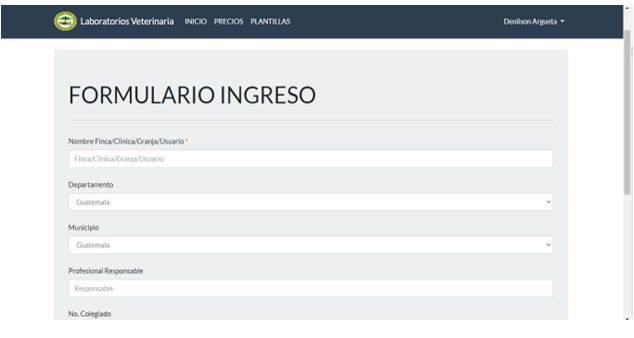
\includegraphics[width=1\linewidth]{images/denilson_01}
\figcaption{Fuente: elaboración propia}

\end{minipage}
\end {flushleft}

Luego de llenar el formulario general, debe escoger en qué laboratorio quiere realizar sus exámenes. Cada uno maneja un formulario diferente para poder solicitar exámenes. Estos formularios los pueden configurar los encargados de los laboratorios en cualquier momento y modificar el orden de las preguntas, agregar otras, modificarlas o eliminarlas. Esto hace que dichos formularios sean dinámicos y puedan ser configurados en cualquier momento.

\begin {flushleft}
\noindent\begin{minipage}[c]{\columnwidth}

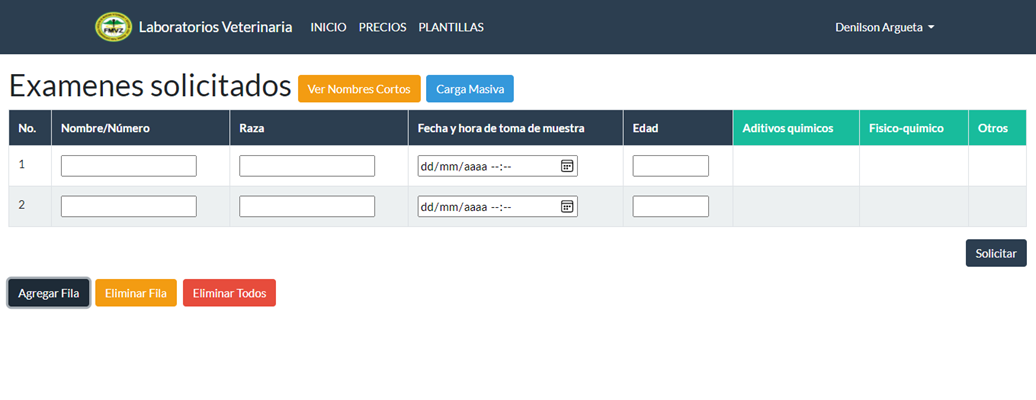
\includegraphics[width=1\linewidth]{images/denilson_02}
\figcaption{Fuente: elaboración propia}

\end{minipage}
\end {flushleft}

Una vez que el cliente llene el formulario del laboratorio de donde quiere solicitar sus exámenes, el sistema le generará una boleta de pago. Con esta puede ir a cualquiera de las agencias de los bancos afiliados a la Universidad de San Carlos de Guatemala a pagar, o bien puede cancelar desde la banca virtual que tengan habilitada dichos bancos.

\begin {flushleft}
\noindent\begin{minipage}[c]{\columnwidth}

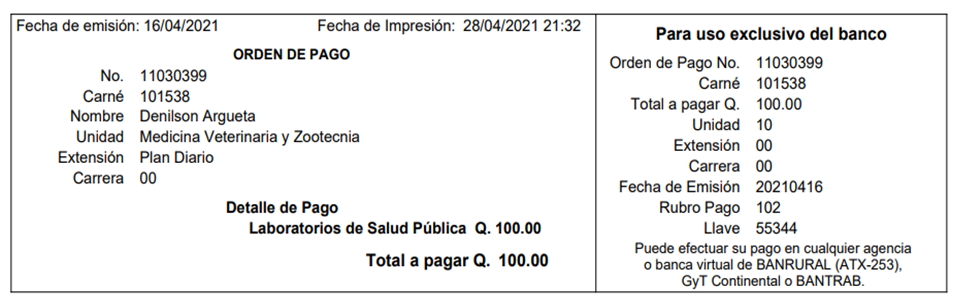
\includegraphics[width=1\linewidth]{images/denilson_03}
\figcaption{Fuente: elaboración propia}

\end{minipage}
\end {flushleft}

Una vez que el cliente haya realizado el pago de sus exámenes, deberá presentarse al laboratorio con las muestras para que se le puedan realizar los exámenes. La persona encargada de recibir las muestras en los laboratorios verifica en el sistema si el cliente ya efectuó el pago y procede a recibirlas. Una vez recibidas, se procede a realizar los exámenes de laboratorio y luego se ingresan los resultados al sistema. El sistema genera el informe de resultados y si el cliente lo solicita, este es enviado al correo que registró

\begin {flushleft}
\noindent\begin{minipage}[c]{\columnwidth}


\includegraphics[width=1\linewidth]{images/denilson_04}
\figcaption{Fuente: elaboración propia}

\end{minipage}
\end {flushleft}

Los encargados de los laboratorios pueden consultar en cualquier momento la cantidad de exámenes que han realizado en un rango de fechas y los ingresos financieros que han tenido.

\hypertarget{conclusiones-1}{%
\section{Conclusiones}\label{conclusiones-1}}

\begin{itemize}
\item
  Con esta aplicación se espera aportar una mejora en los sistemas de la Facultad de Veterinaria, a fin de dar un mejor servicio.
\item
  Con el sistema ahora será posible llevar un mejor control de los ingresos financieros de cada uno de los laboratorios.
\item
  Actualmente, los clientes son notificados de forma inmediata cuando los resultados de los exámenes están listos.
\end{itemize}

\end {multicols}
\medskip
\HRule
\medskip

\hypertarget{cArzudia}{%
\chapter{Gobernanza de la información}\label{cArzudia}}

\begin{center}
\includegraphics[width=1\linewidth]{images/jAzurdia_image1} \end{center}

\begin {multicols}{2}

\hypertarget{resumen-2}{%
\section{Resumen}\label{resumen-2}}

La gobernanza de datos ayuda a realizar una administración adecuada respecto de cualquier información peculiar; los datos de una organización se han convertido en un bien preciado que ayuda a la toma de decisiones y saber de qué manera mejorar un producto o un proceso; la gobernanza de datos ayuda también a hacer un análisis adecuado de datos y brindar información confiable.

\hypertarget{abstract-2}{%
\section{Abstract}\label{abstract-2}}

¿De qué manera ayuda la gobernanza de datos? Nos ayuda al momento en el que una organización crece demasiado y no es capaz de mantener sus datos de forma segura, ya que estos se vuelven complicados. La gobernanza de datos es una combinación de individuos, tecnologías y sistemas que trabajan juntos para proteger los datos de una organización.

\hypertarget{palabras-claves-2}{%
\section{Palabras claves}\label{palabras-claves-2}}

Información, administración, análisis, gestión, beneficio, decisión.

\hypertarget{introducciuxf3n-2}{%
\section{Introducción}\label{introducciuxf3n-2}}

La gobernanza de datos está empezando a introducirse en empresas que desean tener una mejor gestión de datos, para determinar cómo dichos datos determinarán su propio éxito. Cada vez la transformación digital se hace presente y es necesario implementar un modelo que permita organizar y optimizar los procesos, lo cual incidirá en las finanzas, ventas, adquisiciones, producción, entre otros.

\hypertarget{artuxedculo-2}{%
\section{Artículo}\label{artuxedculo-2}}

Una gobernanza de datos es una combinación de individuos, tecnologías y sistemas que trabajan juntos para proteger los datos de una organización; esto garantiza que los mismos sean precisos, completos y fácilmente detectables para los empleados.

Hoy en día los datos se han convertido en el activo corporativo principal y determinan el éxito de un negocio. Realmente los negocios deberán adaptarse a la era digital de forma que los ayude a alcanzar sus objetivos.

La gobernanza de información tiene cuatro pilares elementales:

\begin{itemize}
\item
  Administración de datos: un administrador de datos es el responsable de la información de una organización en colaboración con analistas y administradores de datos; tratan de identificar de qué manera se puede utilizar esta información.
\item
  Calidad de datos: mejorar la calidad de los datos es una actividad constante para una empresa; los mismos deben ser precisos, íntegros y coherentes; esto será señal de que los datos de una organización y su modelo de gobernanza sean exitosos.
\item
  Gestión de datos: establece un conjunto de datos sobre clientes, productos y otras entidades; esto puede garantizar que los datos sean coherentes.
\item
  Casos de uso: este pilar se centra en la manera en que serán utilizados los datos en las aplicaciones de un negocio inteligente y de cómo puede ayudar a una empresa y su entorno a reducir riesgos.
\end{itemize}

Para aplicar una gobernanza de datos en un negocio es necesario definir propietarios de datos y de qué manera los manejarán; se deben establecer políticas de acceso y reglas específicas para que los mismos se mantengan consistentes y actualizados.

\begin {flushleft}
\noindent\begin{minipage}[c]{\columnwidth}

\begin{center}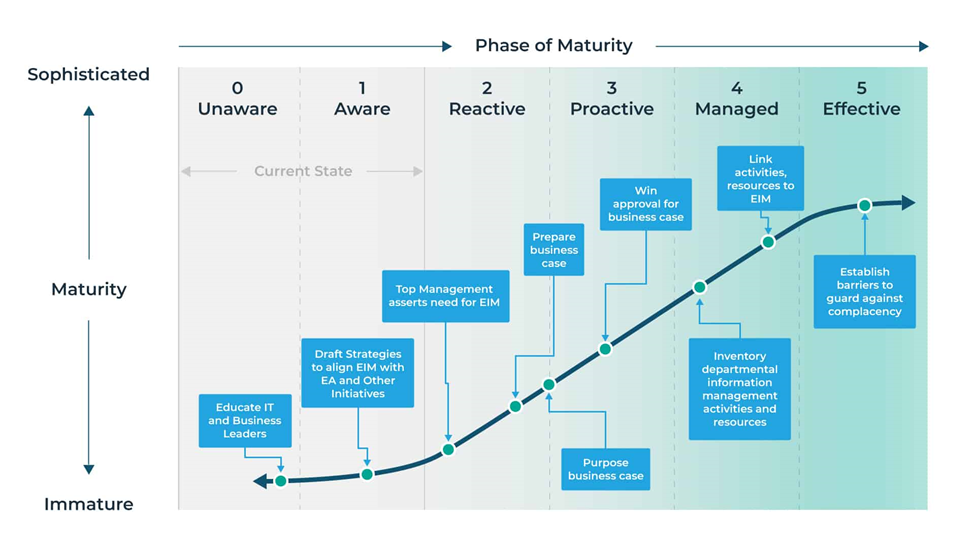
\includegraphics[width=0.8\linewidth]{images/arzudia_01} \end{center}

\figcaption{ Fuente; Gartner (2021). Gobernanza de datos. Recuperado de https://acortar.link/kCsSZB. }

\end{minipage}

\end {flushleft}

También se debe definir cómo y en qué tipo de base serán almacenados estos datos; cada cuánto se les realizará respaldos y cómo serán protegidos. Toda esta información debe mantener un grado de transparencia para las personas interesadas, tales como inversionistas, clientes, entre otros. Finalmente establecer procedimientos de auditoría que aseguren el cumplimiento de las normas del gobierno.

\begin {flushleft}
\noindent\begin{minipage}[c]{\columnwidth}

\begin{center}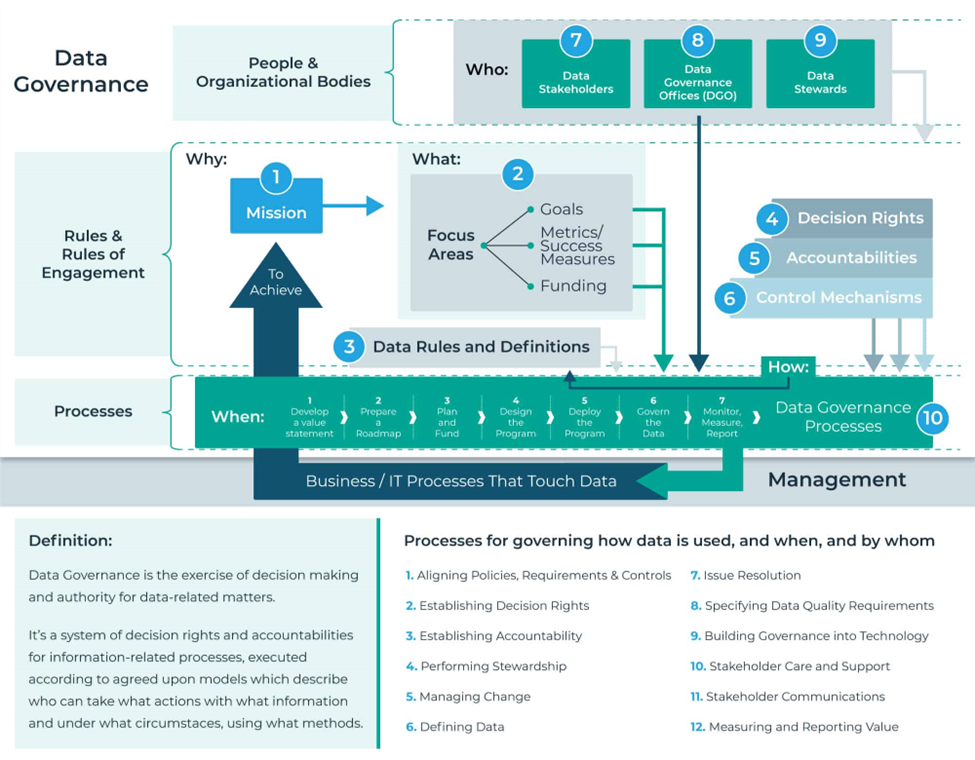
\includegraphics[width=0.8\linewidth]{images/arzudia_02} \end{center}
\figcaption{Profisee (s.f). The Data Governance Institute. Recuperado de https://acortar.link/kCsSZB. }

\end{minipage}

\end {flushleft}

Un ejemplo de la gobernanza de datos es la aplicación ``Openstreetmap'' la cual es un proyecto colaborativo para crear mapas editables y libres. Fue creado por el empresario británico Steve Coast en el 2004 y fue una respuesta, ya que existía una gran cantidad de fuentes de datos geográficos y ninguna estaba relacionada entre sí.

Todos los datos recopilados constituyen el aporte de colaboradores y están disponibles para cualquier persona; por tanto, es posible contribuir con informa-
ción y consultar datos. Actualmente esta aplicación es utilizada por Facebook, MapQuest y FourSquare.

\hypertarget{conclusiones-2}{%
\section{Conclusiones}\label{conclusiones-2}}

\begin{itemize}
\item
  Una gobernanza de datos ayuda al análisis adecuado de los mismos y una visión confiable de la información.
\item
  Este modelo propone definir propietarios, quienes serán encargados de gestionar los datos y mantenerlos actualizados.
\item
  La gobernanza de datos permite mantener un control de los suministros que una empresa adquiere.
\end{itemize}

\hypertarget{referencias-1}{%
\section{Referencias}\label{referencias-1}}

\begin{itemize}
\item
  {[}1{]} {[}Amaresan, S. (2019){]}{[}The Straightforward Guide to Data Governance (DG). Hubspot.{]}. Recuperado de: \url{https://acortar.link/Q6blb1}. {[}Último acceso: 29 de octubre de 2022{]}.
\item
  {[}2{]} {[}Gartner (2021){]}{[}Gartner Keynote: the future of business Is composable{]}. Recuperado de: \url{https://acortar.link/kCsSZB}. {[}Último acceso: 29 de octubre de 2022{]}.
\item
  {[}3{]} {[}PowerData (s.f){]}{[}Data Governance y Data Lake: la política de datos a nuestro favor{]}. Recuperado de: \url{https://acortar.link/bUbJYy}. {[}Último acceso: 28 de octubre de 2022{]}.
\item
  {[}4{]} {[}PowerData (s.f){]}{[}Desmitificando el Data Governance: qué, cuándo, dónde y por qué{]}. Recuperado de: \url{https://acortar.link/FZv23S}. {[}Último acceso: 29 de octubre de 2022{]}.
\item
  {[}5{]} {[}PROFISEE (s.f){]}{[}Data Governance: What, why, how, who \& 15 best practices{]}. Recuperado de: \url{https://acortar.link/kCsSZB}. {[}Último acceso: 29 de octubre de 2022{]}.
\item
  {[}6{]} {[}Prometeus.(s.f){]}{[}Alinea los datos a la estrategia de tu organización, bienvenido al Data Governance. Consultado el 4 de marzo de 2019{]}. Recuperado de: \url{https://acortar.link/kCsSZB}. {[}Último acceso: 29 de octubre de 2022{]}.
\end{itemize}

\end {multicols}
\medskip
\HRule
\medskip

\hypertarget{Estrada}{%
\chapter{Experiencia total}\label{Estrada}}

\begin{center}
\includegraphics[width=1\linewidth]{images/jEstrada_image1} \end{center}

\begin {multicols}{2}

\hypertarget{resumen-3}{%
\section{Resumen}\label{resumen-3}}

En este artículo se describe una de las principales tendencias tecnológicas estratégicas de Gartner para 2021: experiencia total. Esta tendencia combina multiexperiencia, experiencia del cliente, del empleado y del usuario para transformar el resultado empresarial.

\hypertarget{abstract-3}{%
\section{Abstract}\label{abstract-3}}

In this article we will find one of Gartner's top strategic technology trends for 2021, total experience. The total experience combines multi-experience, customer experience, employee experience, and user experience to transform business results.

\hypertarget{palabras-claves-3}{%
\section{Palabras claves}\label{palabras-claves-3}}

Experiencia del cliente, usuario, empleado, UX

\hypertarget{introducciuxf3n-3}{%
\section{Introducción}\label{introducciuxf3n-3}}

Tradicionalmente se han tratado por separado la multiexperiencia, y las experiencias de usuarios, clientes y empleados. Sin embargo, ahora Gartner va un paso más allá e indica que estas deben de conectarse para evolucionar y conseguir una mejor experiencia de todas las partes.

\hypertarget{artuxedculo-3}{%
\section{Artículo}\label{artuxedculo-3}}

El objetivo es mejorar la experiencia general donde se cruzan todas estas piezas, desde la tecnología hasta los empleados, los clientes y los usuarios.

Dado que todas las empresas están tratando de mejorar su experiencia, apostar por la experiencia total puede ofrecer una excelente oportunidad para diferenciarse de la competencia.

\begin {flushleft}
\noindent\begin{minipage}[c]{\columnwidth}

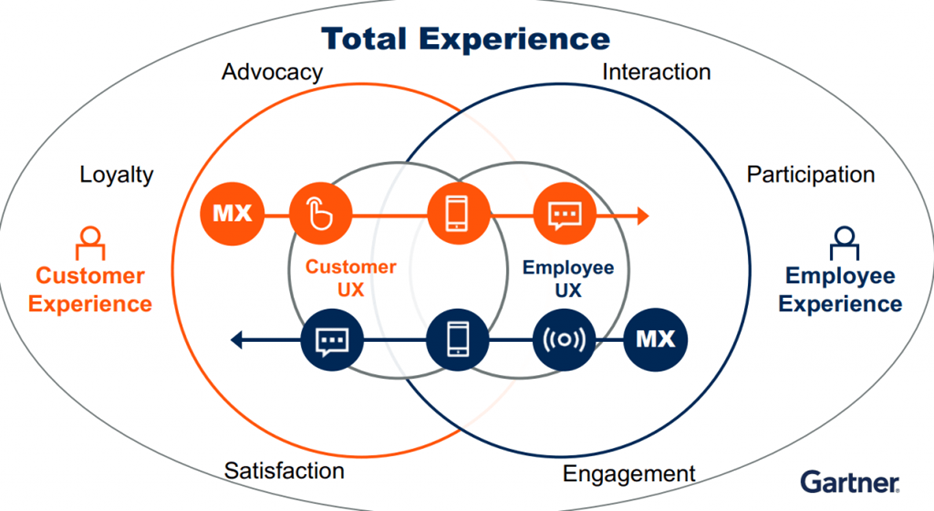
\includegraphics[width=1\linewidth]{images/estrada_01}
\figcaption{Fuente: AuraQuantic (2020). Tendencias tecnológicas y empresariales para el 2021. Recuperado de https://acortar.link/o6KNjS. }

\end{minipage}

\end {flushleft}

En la medida en que las interacciones se vuelven más móviles, virtuales y distribuidas, se hace más necesaria una estrategia de experiencia total que satisfaga por igual a clientes, empleados y usuarios, y para conseguir este objetivo tiene sentido centrarse en una estrategia de mejoras que resulte útil para todos los grupos.

Una encuesta de Gartner, de acuerdo con Paneta (2020) reveló que solo el 13 \% de los empleados está completamente satisfecho con su experiencia. Las organizaciones están realizando importantes acciones para mejorar la experiencia de los empleados, como inversiones de incorporación y rediseño del lugar de trabajo. Aunque estas inversiones mejoran gradualmente, la satisfacción y el compromiso de los empleados, el costo de cumplir con las expectativas cada vez mayores de los empleados es insostenible.

La experiencia del usuario (UX) es la suma de los efectos causados por una persona que utiliza una solución digital. Los esfuerzos de UX se concentran en la experiencia que tienen las personas cuando interactúan con un producto o solución específicos.

La mayoría de las organizaciones grandes, con ingresos de más de mil millones de dólares, tienen más de 50 métricas de CX, algunas hasta 200; todas pertenecientes y administradas por diferentes personas en diversas partes de la organización.

Vale la pena mencionar los tipos de experiencia que pueden darse en una organización:

\begin{itemize}
\tightlist
\item
  La experiencia múltiple: consiste en la experiencia general de determinada marca, producto y/o servicio en varios canales y dispositivos.
\item
  La experiencia del usuario: se refiere al diseño, usabilidad y funcionalidad de su producto o servicio.
\item
  La experiencia del cliente: se refiere al aspecto general, la sensación y la calidad de sus interacciones con los clientes en cada punto de contacto a lo largo de su recorrido.
\item
  La experiencia del empleado: hace alusión al aspecto general, la sensación y calidad de interacciones con los empleados en cada punto de su carrera o permanencia en la empresa, desde la contratación hasta la jubilación.
\end{itemize}

\hypertarget{conclusiones-3}{%
\section{Conclusiones}\label{conclusiones-3}}

Vincular estrechamente todas estas experiencias en lugar de mejorar individualmente cada una en un silo, diferencia a una empresa de la competencia de una manera difícil de replicar, lo que crea una ventaja competitiva sostenible. Esta tendencia permite a las organizaciones capitalizar los disruptores COVID-19, incluidos el trabajo remoto, los clientes móviles, virtuales y distribuidos.

\hypertarget{referencias-2}{%
\section{Referencias}\label{referencias-2}}

\begin{itemize}
\tightlist
\item
  {[}1{]} {[}Panneta, K. (2020){]}{[}Las principales tendencias tecnológicas estratégicas de Gartner para 2021. Consultado el 30 de julio de 2019{]}. Recuperado de: \url{https://acortar.link/A5BK9a}. {[}Último acceso: 29 de octubre de 2022{]}.
\end{itemize}

\end {multicols}
\medskip
\HRule
\medskip

\hypertarget{ramiro}{%
\chapter{Realidad aumentada}\label{ramiro}}

\begin{center}
\includegraphics[width=1\linewidth]{images/jMateo_image1} \end{center}

\begin {multicols}{2}

\hypertarget{resumen-4}{%
\section{Resumen}\label{resumen-4}}

La realidad virtual es una tecnología que ha aumentado considerablemente con ingresos de varios miles de millones de dólares; esto se debe a que la realidad virtual busca reemplazar la realidad del mundo real, simulando las experiencias de un determinado lugar, al cual se le agregan datos o información de una realidad; ha tomado mayor auge en los videojuegos, ya que hace que los jugadores se sumerjan en la virtualidad como si fuese una realidad, la cual por lo general es casi perfecta como la realidad; esto implica una superposición de datos, imágenes, audios y videos sobre la realidad como tal. Puede afirmarse que es potencial porque crea un vinculo con el cliente, presentándole una realidad novedosa que despierta mayor interés y que le hace sentirse apegado y familiarizado con productos y servicios que se ofrecen, ya que no solo verán publicidad plana e impresa, sino que también podrán experimentar físicamente los productos o servicios, lo cual hará que el cliente tenga en cuenta en su memoria su experiencia, la que, en un inicio es muy asombrosa.

\hypertarget{abstract-4}{%
\section{Abstract}\label{abstract-4}}

Virtual reality is a technology that has increased considerably with income of several miles of millions of dollars, this is because virtual reality seeks to replace the reality of the real world, simulating the experiences of a certain place to which data or information is added a reality, it has taken a greater boom in video games since it makes players immerse themselves in virtuality as if it were a reality, which in general is almost perfect as reality, which implies an overlay of data, images, audios, videos about reality as such. So it is potential because it creates a bond with the client by presenting a new reality that arouses greater interest and feels attached and familiar with the products and services that are offered, since they will not only see flat and printed advertising, but they will also be able to physically experiment the products or services which will make the client take into account in his memory his experience which at the beginning is very amazing.

\hypertarget{palabras-claves-4}{%
\section{Palabras claves}\label{palabras-claves-4}}

Datos, imágenes, sentidos, mundo real, interés, publicar, marca, ganancias.

\hypertarget{introducciuxf3n-4}{%
\section{Introducción}\label{introducciuxf3n-4}}

El auge del marketing digital ha hecho que en la actualidad muchas empresas inicien con la investigación y utilización de nuevas técnicas para incrementar la difusión de las diferentes campañas publicitarias, con el fin de llegar a más clientes y atraer un mayor número de personas interesadas en la adquisición de sus productos, aprovechando que la tecnología se ha vuelto una herramienta para facilitar dicha tarea, por lo que el impacto e importancia que se desea es un factor que incidirá en excelentes resultados; de modo que el uso de la realidad aumentada es ideal para realizar las diferentes campañas publicitarias, ya que con ello se logrará despertar mayor interés en los clientes, porque hará que se sientan apegados y familiarizados con productos y servicios que se ofrecen, ya que podrán apreciarlos físicamente; esta asombrosa experiencia, en cierta forma enganchará o mantendrá al cliente fiel a una determinada marca.

\hypertarget{artuxedculo-4}{%
\section{Artículo}\label{artuxedculo-4}}

La realidad aumentada es un conjunto de técnicas que permite sobreponer elementos virtuales sobre nuestra perspectiva de la realidad. Actualmente ha aumentado la demanda; en los últimos años se ha convertido en un negocio que ascendió a la cifra de varios miles de millones de dólares en todo el mundo. La realidad virtual busca reemplazar la realidad mediante el uso de dispositivos que permitan tener una experiencia en otro lugar o simular la presencia, estando en un lugar diferente. Esta tecnología se ha usado en numerosas ocasiones en el mundo de los videojuegos. Con lentes especiales el jugador se puede sumergir a la realidad virtual con total naturalidad.

La realidad aumentada es una forma de la realidad, pero más precisa; por lo que se considera perfeccionada, ya que en ella se agregan imágenes o información realizadas en computadoras, las cuales se ajustan al entorno a través de los sentidos. Un ejemplo de dispositivo de realidad aumentada es el Google glass. Estos lentes permiten conseguir información referente a rutas, clima, negocios, avisos de email, todo sin contaminar la realidad, sino complementándola. Otro ejemplo es el juego Pokémon Go, una aplicación en la que los usuarios caminan por la calle para encontrar Pokémons. Este juego se hizo muy conocido y es el ejemplo ideal para ilustrar cómo se puede usar la realidad aumentada para llegar a mucha gente.

La realidad aumentada hace uso de la tecnología digital para sobreponer información sobre los formatos convencionales de imágenes, vídeos o textos, según sea el objetivo o se necesite. Es decir, consiste en una tecnología en aumento en la que los datos digitales se fusionan con la realidad. Así, esta tecnología superpone datos generados por computadoras sobre el mundo real. Además, según las tendencias y debido al auge de los dispositivos móviles, los usuarios utilizan un smartphone o tablet para explorar el mundo mediante el uso de la realidad aumentada.

La realidad aumentada es considerada actualmente como un potencial de mercado inconcebible. Según un estudio de ESIC, Digi-capital (2017) se espera que consiga un número de clientes que aporten miles de millones de dólares en un futuro muy cercano. La cuota de ingresos de la realidad aumentada se dividirá entre diferentes factores tales como la publicidad, el consumidor, los parques temáticos, el cine o televisión, los E-commerce y hardware, para que se encarguen de representar dicha realidad. Además, ese mismo estudio prevé que la realidad aumentada alcance a mil millones de personas en el mundo entero.

También la realidad aumentada ofrece la oportuni-
dad de crear un vínculo entre la marca y los clientes. Ese vínculo se fortalece mediante la nueva forma de comunicación e interacción con los mismos. Al mismo tiempo que se les da la oportunidad de explorar los productos que ofrece la marca de una forma diferente y posiblemente más cómoda y mejorar el conocimiento de la misma, tanto en relación con los clientes como con los medios de comunicación y difusión. Por lo que se busca ofrecer una experiencia novedosa, que además genere un factor de asombro que por lo general favorezca el interés por la marca.

Por lo tanto, al incrementar el enganche del cliente ofreciendo más información de manera fácilmente accesible, el consumidor se vincula a la marca; práctica que también le contribuye a tener más capacidad de decisión y a optimizar el proceso de venta. Gracias a la realidad aumentada los usuarios no vivirán únicamente una campaña de marketing más. Se trata de vivir una experiencia física a la que hay que vincularla.

Diferenciarse de la competencia es uno de los factores muy importantes; la realidad aumentada incentiva la creatividad y las campañas de marketing de forma distinta. Las empresas tienen la oportunidad de promocionar el servicio o producto de cualquier forma, hasta lograr que el nombre de una marca pase por encima de otras de su mismo sector, además de crear mucho interés con el servicio o producto.

La realidad aumentada favorece el inicio de contactos exclusivos que despierten el interés de los consumidores. De ese modo propicia de modo directo el incremento de visibilidad de la marca y el ascenso de su reputación.

La realidad aumentada busca el requerimiento primordial que se desea de toda campaña de marketing. Sorprender a los usuarios es esencial para que la marca permanezca en la memoria del cliente; así mejora su experiencia de información, evitando la saturación típica de cualquier campaña tradicional.

\begin {flushleft}
\noindent\begin{minipage}[c]{\columnwidth}

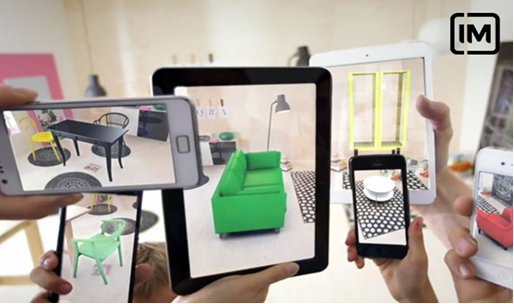
\includegraphics[width=1\linewidth]{images/ramiro_01}
\figcaption{Fuente: IM Digital Business School (2020). Recuperado de https://acortar.link/bYy64b. }

\end{minipage}

\end {flushleft}

\hypertarget{conclusiones-4}{%
\section{Conclusiones}\label{conclusiones-4}}

La realidad aumentada como herramienta de marketing digital es un activo potencial que aumentará considerablemente las ventas en cualquier ámbito que se utilice con mayor creatividad y se explote de la mejor manera las ventajas y utilidades que proporciona esta tecnología.

\hypertarget{referencias-3}{%
\section{Referencias}\label{referencias-3}}

\begin{itemize}
\item
  {[}1{]} {[}Arreguin González, J. F. (2014){]}{[}Realidad aumentada, análisis y aplicaciones{]}. Recuperado de: \url{https://acortar.link/NNJPew}. {[}Último acceso: 30 de octubre de 2022{]}.
\item
  {[}2{]} {[}ESIC. (2017).{]}{[}El futuro de las aplicaciones de realidad aumentada{]}. Recuperado de: \url{https://acortar.link/tTOdTX}. {[}Último acceso: 30 de octubre de 2022{]}.
\item
  {[}3{]} {[} Grupo Garatu It Splutions. (2018){]}{[}Realidad virtual (VR) y realidad aumentada (AR) en las empresas{]}. Recuperado de: \url{https://acortar.link/SafuQJ}. {[}Último acceso: 30 de octubre de 2022{]}.
\item
  {[}4{]} {[}Neosentec (2018){]}{[}Realidad Aumentada. D{]}. Recuperado de: \url{https://acortar.link/TgSfQr}. {[}Último acceso: 30 de octubre de 2022{]}.
\end{itemize}

\end {multicols}
\medskip
\HRule
\medskip

\hypertarget{marco}{%
\chapter{Tendencias tecnológicas 2021}\label{marco}}

\begin{center}
\includegraphics[width=1\linewidth]{images/mChavez_image1} \end{center}

\begin {multicols}{2}

\hypertarget{resumen-5}{%
\section{Resumen}\label{resumen-5}}

Los asistentes virtuales han estado presentes entre nosotros; sin embargo, aún no se ha explotado lo suficiente este campo. Durante estos años se tienen nuevas tecnologías de asistencia virtual más avanzadas, pues son capaces de ejercer como agentes de facturación virtual o agentes virtuales de inteligencia artificial o realidad virtual; hasta pueden llegar a ser asistentes en automóviles autónomos.

\hypertarget{abstract-5}{%
\section{Abstract}\label{abstract-5}}

Virtual assistants have been present among us; however, this field has not yet been exploited enough, during these years, there are new more advanced virtual assistance technologies to come, then, they are capable of acting as virtual billing agents, virtual agents of artificial intelligence or virtual reality can even become assistants in autonomous cars.

\hypertarget{palabras-claves-5}{%
\section{Palabras claves}\label{palabras-claves-5}}

Gartner, cuadrante de Gartner, 5G, Inteligencia artificial

\hypertarget{introducciuxf3n-5}{%
\section{Introducción}\label{introducciuxf3n-5}}

Se mostrarán y evaluarán las tendencias que según Gartner, citado por Jordan (2021) seguirán utilizándose las tecnologías que han estado emergiendo desde el 2010 hasta la fecha; se evaluará la razón del porqué siguen dichas tendencias y el entorno en el cual estas se han estado desarrollando y cuál es la influencia que ejercen sobre las tecnologías.
Se observará que, debido a la situación actual, las tecnologías que están sobresaliendo son aquellas que involucran al distanciamiento, pues el mismo es necesario para preservar la salud de los habitantes y, por ende, tecnologías que involucran automatización de procesos.

\hypertarget{artuxedculo-5}{%
\section{Artículo}\label{artuxedculo-5}}

La Inteligencia artificial IA, realidad extendida RV y el despliegue masivo de la red 5G son las principales tendencias (Rodríguez, 2021).

\begin {flushleft}
\noindent\begin{minipage}[c]{\columnwidth}

\begin{center}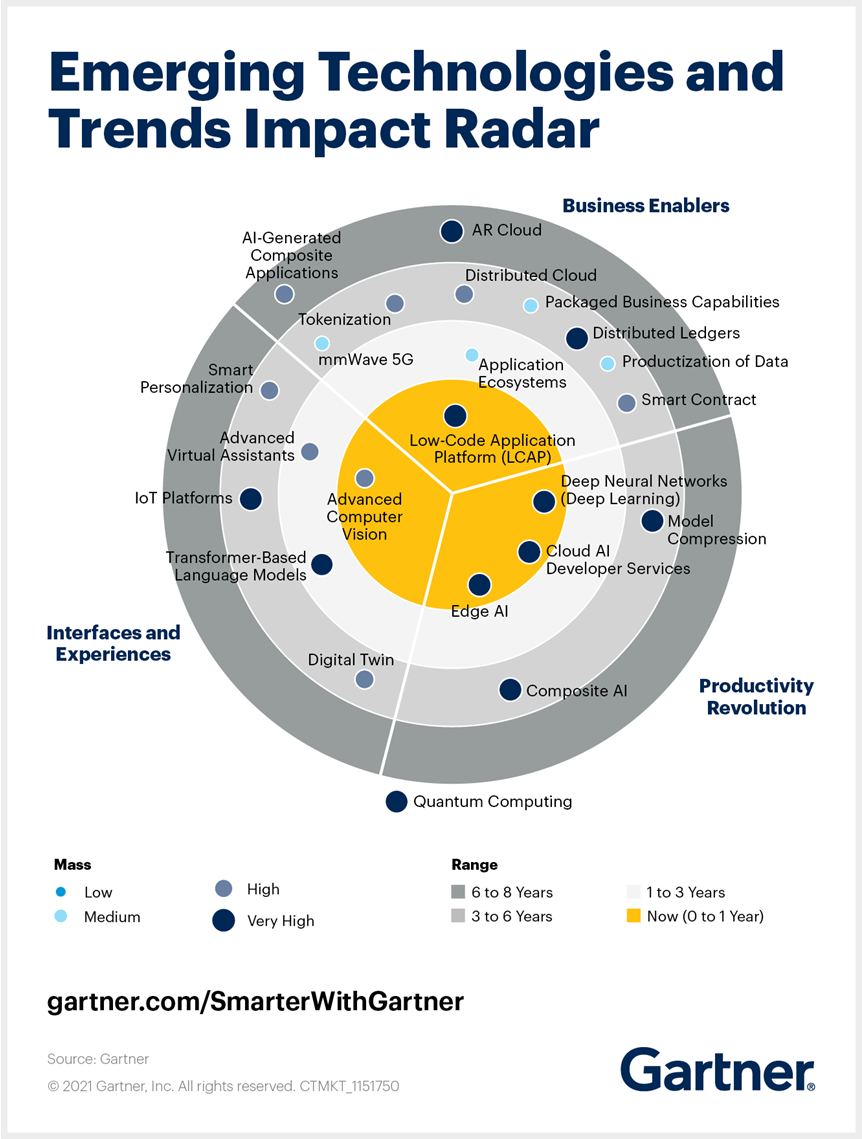
\includegraphics[width=0.9\linewidth]{images/marco_01} \end{center}
\figcaption{Fuente: Gartner (2021), Consultado el 30 de octubre de 2022. Recuperado de https://acortar.link/qIHdxl. }

\end{minipage}
\end {flushleft}

Los asistentes virtuales han estado presentes en nuestro medio, sin embargo, aún no se ha explotado lo suficiente este campo. Durante estos años, nuevas tecnologías de asistencia virtual más avanzados están por venir, pues son capaces de funcionar como agentes virtuales de inteligencia artificial, de facturación virtual o de realidad virtual; hasta pueden llegar a ser asistentes en automóviles autónomos (Jordan, 2021).

Gartner (2021) muestra las 23 tecnologías más impactantes en su Radar de Impacto de Tendencias y Tecnologías, dando a conocer, además de los asistentes virtuales, otras tecnologías en dicho radar. Las tecnologías de este radar se pueden

\begin{itemize}
\item
  Interfaces y experiencias: son aquellas tecnologías que están cambiando el modo en que se interactúa con nuestro alrededor.
\item
  Habilitadores empresariales: son aquellas tecnolo-
  gías que cambian el modo en que operan las empresas, siendo estos los cambios prácticos, procesos, métodos, modelos o funciones.
\item
  Revolución de la productividad: la unión de múltiples tecnologías y tendencias que ayudan a organizaciones a operar de manera más eficiente para resolver problemas que estas tengan (Nguyen, 2021).
\end{itemize}

\textbf{IA}

Por medio de la IA los teléfonos celulares incorporan funciones como reconocimiento facial y sensores biométricos. Por ejemplo, un bot presente en la interacción de una entidad pública y los ciudadanos será capaz de identificar cuál es el trámite que se quiere llevar a cabo (pago de una multa).
En el área de ciberseguridad, permitirán detectar múltiples tipos de ataques y detenerlos sin intervención humana. Gracias a la IA se podrían identificar patrones de forma automática para localizar al atacante.
También hay riesgos, porque la IA permite adaptar un sistema de acuerdo con el comportamiento de cada usuario. TikTok, Instagram y Netflix aplican algoritmos para analizar el comportamiento de los usuarios.

\textbf{Realidad extendida}

La realidad extendida se refiere a una tecnología que permite al usuario experimentar y manipular objetos virtuales a través de interacciones hombre-máquina, gracias a wearables que permiten a la persona realizar acciones con simples gestos.

\textbf{Red 5G}

Se está a la expectativa de que empiece a probarse el Red 5G en Europa, Norteamérica, Asia Oriental y otras regiones desarrolladas. Los estándares serán la banda de 700 MHz con mejor cobertura y 26 GHz que ofrece grandes velocidades y latencias bajas.
La pandemia ha afectado notablemente el despliegue de redes 5G. Sin embargo, ya se han sacado al mercado dispositivos inteligentes que utilizan esta tecnología.

\textbf{Asistentes virtuales avanzados}

Los asistentes virtuales avanzados o AAV por sus siglas o también llamados agentes conversacionales de IA, procesan las entradas humanas para entregar predicciones y decisiones. Están impulsados por una combinación de interfaz de usuario conversacional, proceso de lenguaje natural PNL y técnicas semánticas y de aprendizaje como redes neuronales profundas DNN. Esta tecnología se estima que tiene un tiempo de comercialización: de 1 a 3 años.

\textbf{Transformer-Based Language Models}

Modelo de lenguaje basado en transformadores: son redes neuronales profundas DNN que procesan palabras como secuencias en una oración. Esta tecnología también mejora la traducción, transcripción y generación de lenguaje natural, estando entrenados en enormes conjuntos de datos de miles de millones de frases. Esta tecnología también estima un tiempo de comercialización de 1 a 3 años.
Capacidades empresariales empaquetadas: permiten a las organiza-
ciones crear experiencias personalizadas compuestas a partir de componentes de aplicaciones que compran o crean. Para admitir el negocio componible los proveedores de tecnología deben ofrecer capacidades empresariales empaquetadas que representen un conjunto bien definido de características empresariales que sean reconocibles como tales por un usuario empresarial. Esta tecnología estima un tiempo de comercialización de 3 a 6 años.

\textbf{Nube de AR}

Es la nube de realidad aumentada que permite la unificación de mundos físicos y digitales mediante la entrega de contenido digital persistente, colaborativo y contextual superpuesto en personas, objetos y ubicaciones, para proporcionar a las personas información y servicios directamente vinculados con todos los aspectos de su entorno físico. Esta tecnología tiene un tiempo de comercialización de 6 a 8 años.

\hypertarget{conclusiones-5}{%
\section{Conclusiones}\label{conclusiones-5}}

Los avances tecnológicos seguirán con la tendencia que ha estado teniendo la inteligencia artificial; la realidad extendida y el despliegue de la red 5G se encuentran entre las principales tendencias. Se estima que muy pronto los asistentes virtuales tendrán más protagonismo. En el área de ciberseguridad, los algoritmos permitirán detectar múltiples tipos de ataques y detenerlos sin intervención humana.

\textbf{Discusión de resultados}

Antes de darse la problemática de la pandemia, según Gartner, citado por Jordan (2021), las tecnologías que estaban en tendencia eran muchas, pero, con la actual modalidad de trabajo maduraron sobre otras tecnologías aquellas que ayudan a la población a laborar alejados de las demás personas o en un ambiente abierto diferente a como solía ser normal.

\hypertarget{recomendaciones}{%
\section{Recomendaciones}\label{recomendaciones}}

El estudio sobre el conocimiento de las tendencias tecnológicas es para aquellas empresas que desean un cambio frente a las situaciones de cambio de su cliente y también para aquellas personas con negocio pequeño o emprendedores, para empezar con las tecnologías que permitan sobrellevar la situación del mercado actual.

\hypertarget{referencias-4}{%
\section{Referencias}\label{referencias-4}}

\begin{itemize}
\item
  {[}1{]} {[}Jordan, B. (2021){]}{[}5 Emerging Technologies Explained by Gartner Experts{]}. Recuperado de: \url{https://acortar.link/jHo8Aq}. {[}Último acceso: 30 de octubre de 2022{]}.
\item
  {[}2{]} {[}Nguyen, T. (2021). {]}{[}4 Impactful Technologies from the Gartner Emerging Technologies and Trends Impact Radar for 2021{]}. Recuperado de: \url{https://acortar.link/MZOU3i}. {[}Último acceso: 30 de octubre de 2022{]}.
\item
  {[}3{]} {[}Rodríguez, A. (2021){]}{[}El 2021 promete tres hitos tecnológicos. El Comercio. Consultado el 3 de marzo de 2021{]}. Recuperado de: \url{https://acortar.link/TUnoBC}. {[}Último acceso: 30 de octubre de 2022{]}.
\end{itemize}

\end {multicols}
\medskip
\HRule
\medskip

\hypertarget{cJuarez}{%
\chapter{¿Internet de los comportamientos como monitoreo de protocolos de salud?}\label{cJuarez}}

\begin{center}
\includegraphics[width=1\linewidth]{images/mSic_image1} \end{center}

\begin {multicols}{2}

\hypertarget{resumen-6}{%
\section{Resumen}\label{resumen-6}}

El Internet de los comportamientos es una de las tecnologías de estrategia que se pondrán de moda para el año 2021, según Gartner.

El Internet of Behavior puede llegar a ser una solución muy útil para la nueva situación de la humanidad: COVID-19. Cada compañía quiere seguridad y lineamientos para la ``nueva realidad''. ¿Qué pasa si la tecnología pudiera resolver este problema? Sí, puede ser real si la empresa usa nueva tecnología como sensores, o recolectando datos y observando el comportamiento de sus empleados. ¿Cómo? Con esta nueva tecnología de Gartner: Internet of Behavior.

\hypertarget{abstract-6}{%
\section{Abstract}\label{abstract-6}}

One of the Gartner's top strategic technology trends for 2021.
Internet of Behaviors could be a very useful solution for new world's situation: COVID19. Every company wants security and guidelines for ``new reality''. What if technology could solve this problem? Yes, it could be real if the company use new-tech, like sensors or recolecting data and watch the behavior of its employees. How? With this new Gartner's trend: Internet of Behavior.

\hypertarget{palabras-claves-6}{%
\section{Palabras claves}\label{palabras-claves-6}}

COVID-19, internet del comportamiento, tecnología emergente, internet de las cosas.

\hypertarget{introducciuxf3n-6}{%
\section{Introducción}\label{introducciuxf3n-6}}

Hoy en día debido a la pandemia que se ha presentado en el mundo, COVID-19, muchas empresas, para seguir sobreviviendo recurren a la necesidad de continuar con sus labores y con esto surgen nuevos problemas como buscar la manera de controlar que sus empleados cumplan con el protocolo de salud establecido; esto puede llegar a ser un proceso que requiere mucha observación; dejar esa tarea en manos de una persona significaría más gastos de lo considerado; para esto el Internet of Behavior puede ser una gran alternativa, ya que hace uso de sensores que permiten analizar comportamientos y llevar monitoreo de los mismos.

\hypertarget{artuxedculo-6}{%
\section{Artículo}\label{artuxedculo-6}}

Recordando el Internet of Things
Es importante partir desde el concepto del Internet of Things (IoT) o Internet de las cosas; este consiste en una serie de dispositivos conectados a una misma red de internet, que interactúan entre ellos para recopilar información del usuario (Johnson, 2020). Estos datos recaudados pueden ser utilizados por las compañías para un estudio de mercadeo que signifique un aporte significativo al área de salud, para personalizar contenido al usuario.
El IoT es escalable, ya que durante el año 2019 se encontraban 27 millones de dispositivos conectados al internet, mientras que para el 2020 fueron 75 billones (Kidd, 2020).
El Internet of Behavior
Ahora bien, para hablar del Internet of Behaviors o Internet del comportamiento, se dice que es algo escalable o extensión del IoT, tal y como se puede apreciar en la figura 8.1.

\begin {flushleft}
\noindent\begin{minipage}[c]{\columnwidth}

\begin{center}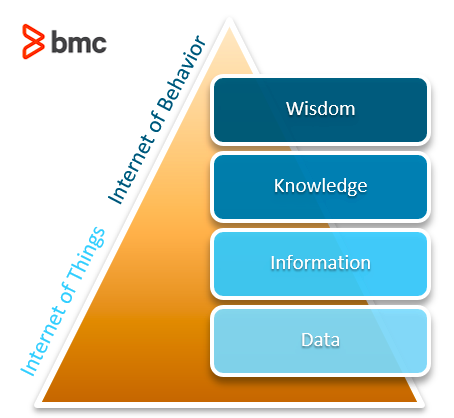
\includegraphics[width=0.8\linewidth]{images/mariana} \end{center}
\figcaption{Fuente:  BMC Blogs (2020). Internet of Behavior. Recuperado de https://acortar.link/OEaj27. }

\end{minipage}

\end {flushleft}

En el triángulo anterior se representa la manera en la que el Internet of things es la base del Internet of Behavior y cómo cada uno de los dos grandes conceptos envuelven otros útiles para soluciones digitales. El Internet of Behavior es una combinación de tecnología, análisis de datos y ciencia del comportamiento. Esta última, a su vez, se subdivide en emociones, decisiones y argumentos, desde la perspectiva del ser humano.

Volviendo al concepto de la escalabilidad del IoT y si este es la base del Internet of Behavior, se puede decir que existe codependencia en el crecimiento de ambos. Por ejemplo: si se utiliza una aplicación en un dispositivo móvil que sea capaz de llevar el control de dieta alimentaria, patrón de sueño, ritmo cardíaco, nivel de azúcar en la sangre y muchas otras observaciones de este tipo, la recolección de datos se le deja al IoT, mientras que al Internet of Behavior le corresponde un análisis profundo de los hábitos que esta aplicación sea capaz de llevar. Esto constituye un aspecto positivo, ya que pueden lograrse mejoras en relación con los hábitos personales, para un mejor rendimiento y desarrollo saludable (Panetta, 2020).

Aplicaciones del Internet of Behavior:
Gartner ha desarrollado una predicción que señala que para el año 2023 las actividades humanas podrán ser rastreadas digitalmente con IoT en compañía del Internet of Behavior, beneficiando de esta manera a un 40 \% de la población a nivel mundial (Costello, K. y Rimol, M., 2020).

Algunas aplicaciones del Internet of Behavior pueden destacar un monitoreo de hábitos de higiene que propicien el seguimiento de los nuevos estándares de salud impuestos en diferentes campos. Por ejemplo, monitorear el uso correcto de mascarillas en empresas, verificación de la frecuencia con que el personal de salud ejerce el acto de desinfección de manos, entre otros. Todo esto con ayuda de sensores, recolección de datos y análisis del comportamiento de quienes estén siendo observados. De esta manera, el Internet of Behavior es una gran solución factible que vale la pena implementar.

\hypertarget{conclusiones-6}{%
\section{Conclusiones}\label{conclusiones-6}}

\begin{itemize}
\item
  El Internet of Behavior es una tendencia que puede llegar a tener mucho auge para el año 2021.
\item
  Analizar el comportamiento del ser humano a través de medios tecnológicos es algo que se puede aprovechar para su mismo desarrollo.
\item
  Utilizar Internet of Behavior en empresas es algo positivo para su crecimiento y control.
\item
  El Internet of Behavior es escalable.
\end{itemize}

\hypertarget{referencias-5}{%
\section{Referencias}\label{referencias-5}}

\begin{itemize}
\item
  {[}1{]} {[}Chrissy, C. (2020). {]}{[}What is the Internet of Behaviors?{]}. Recuperado de: \url{https://acortar.link/ScRnDN}. {[}Último acceso: 30 de ocubre de 2022{]}.
\item
  {[}2{]} {[}Costello, K. y Rimol, M. (2020){]}{[}Gartner Unveils Top predictions for it organizations and users in 2020 and beyond{]}. Recuperado de: \url{https://acortar.link/mCKdeg}. {[}Último acceso: 30 de octubre de 2022{]}.
\item
  {[}3{]} {[}Johnson, J. (2020). {]}{[}What Is the Internet of Things (IoT)? {]}. Recuperado de: \url{https://acortar.link/GmSp7G}. {[}Último acceso: 5 de mayo de 2021{]}.
\item
  {[}4{]} {[}Panetta, K. (2020){]}{[}Gartner Top Strategic Technology Trends for 2021{]}. Recuperado de: \url{https://acortar.link/fKiHUw}. {[}Último acceso: 30 de octubre de 2022{]}.
\end{itemize}

\end {multicols}
\medskip
\HRule
\medskip

\hypertarget{tun}{%
\chapter{Tecnologías del distanciamiento social}\label{tun}}

\begin{center}
\includegraphics[width=1\linewidth]{images/mTun_image1} \end{center}

\begin {multicols}{2}

\hypertarget{resumen-7}{%
\section{Resumen}\label{resumen-7}}

El distanciamiento social para muchas personas significó un cambio de hábito en relación con la costumbre de estar cerca de familiares y amigos; como también de los empleados que laboran desde hace varios años en determinada empresa. En la mayoría de los países las normas de distanciamiento son reglas que deben cumplirse a cualquier hora y en cualquier lugar público para evitar el contagio del Covid-19. El cumplimiento de dichas normas ha sido posible con la ayuda de tecnologías y sus herramientas automatizadas, desde prototipos de dispensadores de gel hasta softwares que indican en tiempo real a qué distancia nos encontramos de las otras personas, así como también los equipos de cómputo y programas que ayudan a que los empleados, comercios y empresas en general, laboren desde cualquier lugar sin ningún problema.

\hypertarget{abstract-7}{%
\section{Abstract}\label{abstract-7}}

Social distancing for many people meant a change of habit in relation to the habit of being close to family and friends; as well as the employees who have been working for several years in a certain company. In most countries, distancing rules are rules that must be followed at any time and in any public place to avoid the spread of Covid-19. All this was possible with the help of the technologies and their automated tools that exist today, from prototypes of gel dispensers to software that tell us in real time how far we are from other people, as well as the equipment of computing and programs that help employees, businesses, and companies in general to work from anywhere without any problem, complying with the rules proposed in a country.

\hypertarget{palabras-claves-7}{%
\section{Palabras claves}\label{palabras-claves-7}}

Robótica, Softwares, innovación, Home office, accesibilidad.

\hypertarget{introducciuxf3n-7}{%
\section{Introducción}\label{introducciuxf3n-7}}

Para continuar con la misma calidad de vida en tiempos de pandemia, la población y empresas tecnológicas han ofrecido opciones diversas para dar solución a esta problemática. El distanciamiento social es parte de las restricciones del gobierno para evitar contagios; es por eso que se han puesto en marcha proyectos y prototipos utilizando las herramientas que ayudan a mantener esta restricción y que son muy eficientes para la población, tales como el uso de robots que miden la temperatura y proporcionan gel con la ayuda de la inteligencia artificial, softwares que son capaces de medir el distanciamiento en lugares con personas alrededor utilizando la tecnología 5g, entre otras soluciones que las personas han creado de acuerdo con sus necesidades para mantener segura a su familia y amigos, así como también realizar las actividades cotidianas, sin romper o incumplir las reglas dadas en un gobierno.

\hypertarget{artuxedculo-7}{%
\section{Artículo}\label{artuxedculo-7}}

Con la llegada de la pandemia del Covid -19, poco a poco se ha dado un proceso de adaptación a las nuevas restricciones; sin embargo, eso no significa que dicha adaptación haya sido fácil, ya que se debe mantener una distancia física estricta para evitar la propagación de los contagios en los entornos de trabajo. Para los profesionales de primera línea de los sectores de la salud, seguridad pública, transporte o logística, está siendo especialmente complicado mantener esa separación de metro y medio o dos metros, mientras siguen trabajando y ofreciendo servicios esenciales, por lo que a continuación se presentan las tecnologías que pueden mejorar esta situación:

\begin{itemize}
\item
  Inteligencia artificial: es la habilidad de una máquina de presentar las mismas capacidades que los seres humanos, como el razonamiento, aprendizaje, creatividad y capacidad de planear.
\item
  Internet de las cosas: IoT es una interconexión de dispositivos y objetos a través de una red (bien sea privada o Internet, la red de redes), donde todos ellos podrían ser visibles e interaccionar.
\item
  Tecnología 5G: esta nueva tecnología móvil aumentará la velocidad de conexión, reducirá al mínimo la latencia (el tiempo de respuesta de la web) y multiplicará exponencialmente el número de dispositivos conectados. En otras palabras: podrá estarse conectado a todo, todo el día, y en el menor tiempo posible.
\item
  Apps y plataformas web.
\item
  Otras soluciones de automatización inteligente.
\end{itemize}

Para tener una mejor idea de por qué estas tecnologías han sido de ayuda en la situación en la que encuentra el mundo, se presentan ejemplos muy valiosos que utilizan las tecnologías ya mencionadas.

\begin {flushleft}
\noindent\begin{minipage}[c]{\columnwidth}

\begin{center}
\includegraphics[width=1\linewidth]{images/tum01} \end{center}
\figcaption{Fuente: Canal de YouTube Open Sistemas. Recuperado de: https://acortar.link/tb0h7V}

\end{minipage}
\end {flushleft}

\begin {flushleft}
\noindent\begin{minipage}[c]{\columnwidth}

\begin{center}
\includegraphics[width=0.95\linewidth]{images/tum02} \end{center}
\figcaption{Fuente: Canal de YouTube INSITE S.A.S Recuperado de: https://acortar.link/FSqvO0.}

\end{minipage}
\end {flushleft}

Robot Covid-19:

\begin {flushleft}
\noindent\begin{minipage}[c]{\columnwidth}

\begin{center}
\includegraphics[width=1\linewidth]{images/tum4} \end{center}
\figcaption{Fuente: Canal de YouTube Vodafone Empresas.  Recuperado de:  https://acortar.link/FSqvO0}

\end{minipage}
\end {flushleft}

A continuación, se presenta otro modelo de automatización inteligente:

\begin {flushleft}
\noindent\begin{minipage}[c]{\columnwidth}

\begin{center}
\includegraphics[width=1\linewidth]{images/tum5} \end{center}
\figcaption{Fuente: Canal de YouTube BBC World Service. Recuperado de:  https://acortar.link/7sjsiy. }

\end{minipage}
\end {flushleft}

\hypertarget{conclusiones-7}{%
\section{Conclusiones}\label{conclusiones-7}}

\begin{itemize}
\item
  Para mantener un distanciamiento social adecuado con cada una de las personas en los lugares con mucha afluencia es importante hacer uso de la tecnología, porque son innovaciones que utilizan inteligencia artificial junto con robótica para hacer más preciso el cálculo de la distancia adecuada establecida.
\item
  Todas las tecnologías que ayudan a mantener el distanciamiento social son parte del inicio para resolver una problemática que surgió con la pandemia del Covid-19; por eso no deben dejarse de utilizar, ya que también podrán resolverse otras problemáticas que vayan surgiendo. Es conveniente que se apliquen de la mejor manera para continuar innovando en el campo de la tecnología.
\end{itemize}

\hypertarget{referencias-6}{%
\section{Referencias}\label{referencias-6}}

\begin{itemize}
\tightlist
\item
  {[}1{]} {[}Garzón, K.2020){]}{[}Tecnologías que ayudan al distanciamiento social{]}. Recuperado de: \url{https://acortar.link/fxQNEJ}. {[}Último acceso: 30 de octubre de 2022{]}.
\end{itemize}

\end {multicols}
\medskip
\HRule
\medskip

\hypertarget{widvin}{%
\chapter{Computación que mejora la privacidad}\label{widvin}}

\begin{center}\includegraphics[width=1\linewidth]{images/wQuiñonez_image1} \end{center}

\begin {multicols}{2}

\hypertarget{resumen-8}{%
\section{Resumen}\label{resumen-8}}

La seguridad brinda la integridad de los datos que se utilizan en la red por medio de distintos mecanismos, herramientas y tecnologías que la ofrecen cuando el usuario se conecta a la red de internet.

\hypertarget{palabras-claves-8}{%
\section{Palabras claves}\label{palabras-claves-8}}

Computación, privacidad, digital, tecnologías, blockchain, confidential AI.

\hypertarget{introducciuxf3n-8}{%
\section{Introducción}\label{introducciuxf3n-8}}

La privacidad es un derecho que todos tenemos; pero en la actualidad se encuentra vulnerable en diversos sitios que frecuentamos en internet. De alguna manera podemos blindarnos de los ataques o la exposición de nuestra privacidad, pero en el mayor de los casos no somos conscientes de ello. Ahí entran las tecnologías y estándares que nos ayudan a mejorar la experiencia en la red. Tanto a nivel físico y lógico estamos expuestos; por ello se utilizan las siguientes tecnologías: el blockchain puede ser una solución accesible para almacenar información de datos inmutables, pero existen otros estándares importantes como la criptografía, que cada día que pasa tiene mayor impacto en la sociedad.

\hypertarget{artuxedculo-8}{%
\section{Artículo}\label{artuxedculo-8}}

Antes de hacer referencia a la privacidad debemos hacernos la pregunta: ¿qué tan seguros estamos en relación con la información que compartimos con las demás personas que intervienen en nuestro entorno? Existen diversas formas de ver la privacidad en internet: está la que se da a nivel de usuario la cual está más expuesta debido a la corriente de pensamiento que las redes sociales vinieron a implantar en nuestra sociedad. Luego está la computación, las tecnologías y las metodologías que se pueden implementar en las operaciones a nivel de desarrollo.

Visto desde el usuario final existen tecnologías que ayudan a proteger nuestra información de terceros y a mejorar la privacidad mientras navegamos por la red. El proxy es una herramienta eficaz, aunque no tan confiable, ya que existen muchas compañías que dicen prestar el servicio gratuitamente, pero nuestros datos pueden ser realmente la moneda de pago. Otra tecnología es una Virtual Private Network (VPN) que provee al usuario de una transferencia de sus servicios a un servidor ubicado en otra parte del mundo, encriptando cada información que es transmitida desde el usuario al servidor, que es quien se conecta a la red. Una VPN también provee el servicio del cambio de IP para enmascarar la ubicación final del usuario.

Ahora, al hablar de tecnologías que brindan esa privacidad a nivel de desarrollo pueden citarse las siguientes: Blockchain technology, Confidential AI, Confidential data analytics, Secure hardware design, Side-Chanel resilience, Software security and memory safety y Verified security and cryptography.

\textbf{Hablemos de Blockchain}

Es un registro consensuado donde todos los bloques contienen la misma información; no se puede modificar un registro dentro de la estructura, ya que se encuentran encriptados los registros para que sean inmutables y perduren todo el tiempo. Básicamente, se tiene la idea de que la tecnología Blockchain viene ligada intrínsecamente a las criptomonedas, pero sus usos y aplicaciones pueden ser diversos. Se puede utilizar en bancos para registrar cada transacción y asegurar su atomicidad durante todo el tiempo. También se puede encontrar en contratos inteligentes para registrar cada movimiento del trámite. Existen tres diferentes tipos de blockchain: públicos, privados e híbridos. Como sus nombres lo indican lo único que los diferencia es el nivel de acceso que se puede tener sobre cada estructura. En los públicos todos pueden ver los registros de transacciones, mientras que en los privados solo se puede acceder con una verificación previa.

\textbf{Confidential AI \& Confidential data Analytics}

La inteligencia artificial es una herramienta muy importante en la industria tecnológica. Existen plataformas que brindan el servicio de integridad en las pruebas y desarrollo dentro de la múltiple colaboración para que los modelos sean precisos y no puedan ser vulnerados. Este punto de confidencialidad entre los modelos de Machine learning utilizados para AI es muy importante, ya que se manejan grandes cantidades de datos que pueden ser sensibles a la generación de resultados inesperados.

El análisis confidencial se refiere a una parte más metodológica para la empresa, donde se puede analizar el nivel de impacto de los datos que se manejan y cuál es su prioridad de encriptación. Los datos de nivel 1, que se refieren a información sensible del usuario, cliente o empleado, deberían ser encriptados con mayor prioridad. Los datos que se utilizan a nivel interno son de menor prioridad para la encriptación.

\textbf{Secure Hardware Design \& Software Design}

Cuando se habla de seguridad del diseño de hardware en general se hace referencia a la incorpora-
ción de la seguridad adecuada en el diseño de los componentes de cómputo en todo el ciclo de desarrollo del producto, generando soluciones que puedan respaldar esa seguridad a futuro para el software. El buen diseño de placas y actualizaciones constantes del firmware hace que se brinde esta seguridad. Pero si el hardware tiene que brindar la seguridad necesaria al usuario, también el software debe hacerlo. Mediante la implementación de buenas prácticas de programación puede evitarse dejar puertas abiertas para los atacantes.

\textbf{Side-channel resilience}
Este método de hackeo es uno de los más peligrosos en la actualidad porque obtiene la información de un sistema informático mediante el análisis de parámetros físicos. Una de las formas de contrarrestar estos ataques es monitorear dónde están esas vulnerabilidades mediante software eficaz o reducir las emisiones de estos parámetros físicos mediante un aislamiento del equipo de su entorno.

A continuación, se presentan modelos de protección de datos que pueden utilizarse:

\begin {flushleft}
\noindent\begin{minipage}[c]{\columnwidth}

\includegraphics[width=1\linewidth]{images/wQuiñonez_image2}
\figcaption{Fuente: Experiencia del usuario en móviles de Huawei. https://acortar.link/6tw1fU }

\end{minipage}
\end {flushleft}

\begin {flushleft}
\noindent\begin{minipage}[c]{\columnwidth}

\includegraphics[width=1\linewidth]{images/wQuiñonez_image3}
\figcaption{Fuente: Updown.com. Recuperado de https://acortar.link/GSkpum}

\end{minipage}
\end {flushleft}

\begin {flushleft}
\noindent\begin{minipage}[c]{\columnwidth}

\includegraphics[width=1\linewidth]{images/wQuiñonez_image4}
\figcaption{Fuente: Redeszone. Recuperado de https://acortar.link/djeUik}

\end{minipage}
\end {flushleft}

\hypertarget{conclusiones-8}{%
\section{Conclusiones}\label{conclusiones-8}}

\begin{itemize}
\item
  Brindar seguridad tanto en el diseño del hardware como en el software, mejora la privacidad del usuario final.
\item
  El blockchain es una opción útil para almacenar información que el usuario requiere que no se manipule con facilidad.
\end{itemize}

\hspace{1cm}

\begin{itemize}
\tightlist
\item
  Todo punto de seguridad para el usuario viene a otra capa de blindaje contra ataques externos.
\end{itemize}

\hypertarget{referencias-7}{%
\section{Referencias}\label{referencias-7}}

\begin{itemize}
\item
  {[}1{]} {[}Learn Blockchain (2020){]}. {[}Último acceso: 30 de octubre de 2022{]}.
\item
  {[}2{]} {[}Red Seguridad (2021){]}{[}El gran desafío de la ciberseguridad en el sector sanitario{]}. Recuperado de: \url{https://acortar.link/1FtaRb}. {[}Último acceso: 30 de octubre de 2022{]}.
\item
  {[}3{]} {[}Tech Blog (2021. Hiperciencia){]}. Recuperado de: \url{https://acortar.link/0G2HQp}. {[}Último acceso: 30 de octubre de 2022{]}.
\end{itemize}

\end {multicols}
\medskip
\HRule
\medskip

\hypertarget{mayra}{%
\chapter{La importancia de las Prácticas Profesionales}\label{mayra}}

\begin{center}
\includegraphics[width=1\linewidth]{images/MscMayra_02} \end{center}

\begin {multicols}{2}

\hypertarget{resumen-9}{%
\section{Resumen}\label{resumen-9}}

Las necesidades de la sociedad son cada vez más específicas, lo que significa que la práctica profesional debe estar encaminada hacia una sola dirección: ser eficiente y capaz de desenvolverse en el mundo laboral.

Las prácticas profesionales son la primera experien-
cia de los futuros profesionales y su entrada al mundo laboral. La experiencia que brindan las prácticas es una fuente de inspiración para muchos estudiantes y representa una oportunidad para enfrentar desafíos, trabajar en equipo y demostrar sus aptitudes.

Se puede decir que la práctica profesional es también el proceso en el cual el estudiante se acerca más al ámbito laboral y va de la mano con las experiencias y conocimientos que ha adquirido en el proceso educativo, para aplicar todos los conocimientos.

Las prácticas profesionales son el primer peldaño en tu carrera profesional y una posible puerta a un futuro empleo. Las prácticas profesionales son sin duda alguna una de las experiencias más valiosas dentro del proceso de estudios.

\hypertarget{palabras-claves-9}{%
\section{Palabras claves}\label{palabras-claves-9}}

Práctica profesional, habilidades, características, experiencia, pasantía, íterns.

\hypertarget{introducciuxf3n-9}{%
\section{Introducción}\label{introducciuxf3n-9}}

La práctica profesional es un proceso muy importante para todo estudiante, porque es el espacio donde se evidencia lo aprendido en el ámbito académico. Es el espacio donde el estudiante pone en marcha todos sus conocimientos por medio de la práctica. Este proceso es importante tanto para el estudiante como para la Universidad, porque aquí es donde se refleja lo aprendido y lo enseñado.

Existen diferentes tipos de prácticas; se clasifican según el área de especialización, las horas destinadas a esta, el tipo de empresa en el cual se realizará, al igual que el nivel de empoderamiento que se le otorga. Son muchas las oportunidades de crecimiento que ofrecen las prácticas; por esto es totalmente fundamental saber si son relevantes o no, y sobre todo saber si influyen en el futuro desempeño profesional.

\hypertarget{artuxedculo-9}{%
\section{Artículo}\label{artuxedculo-9}}

En el mundo laboral, actualmente, es necesario tener un buen rendimiento debido a que las empresas exigen profesionales eficientes para desarrollar los procesos necesarios que permitan alcanzar los objetivos de la compañía. Para tener un buen rendimiento laboral existen varios determinantes: en primer lugar, se encuentra la formación académica, pues es de suma importancia la adquisición de conocimientos obtenidos en la universidad; luego el desarrollo de competencias tanto técnicas como transversales; estas no son aprendidas solamente en la universidad, sino que también existe otro mundo donde son potenciadas y/o adquiridas; este mundo es el de las prácticas (Ferreyra, 2007).

Sacristán (2007) y Peñaloza (2005), refieren que la práctica profesional busca ser un espacio para la aplicación de los conocimientos adquiridos, en aras de proporcionar un beneficio institucional, involucran la investigación permanente y la acción práctica. Pretenden generar conocimientos, productos y aportes significativos a las organizaciones que brindan la oportunidad de recibir estudiantes para el desarrollo de sus prácticas profesionales.

Para De La Vega y Arakaki (2011, p.~77) ``las prácticas profesionales constituyen un componente esencial de la formación de los estudiantes de educación superior\ldots{} tendiéndose así un puente entre la teoría y la práctica, entre la etapa formativa y el ingreso al mercado laboral''. Los aprendizajes que se desprenden de la ejecución de prácticas profesionales poseen componentes de índole actitudinal, ético y afectivo, que no es posible obtenerlos en las aulas de clase, sino desde la vivencia en situaciones laborales reales, por parte de los estudiantes. A través de los mencionados componentes se consolida una formación más integral; los participantes pueden tener una visión más global de la realidad, en tanto que se le abre paso a la intervención de variables no controladas ante las cuales es menester proponer soluciones, y al mismo tiempo se valida la instrucción teórica recibida.

Según Castellanos (2008, p.~3), ``la práctica profesional es el ejercicio profesional inicial, guiado y supervisado por asesores externos y tutores, donde se aplican en forma directa los conocimientos adquiridos en el proceso formativo del estudiante''. ``La Práctica Profesional constituye una actividad de estudio y trabajo, que, bajo régimen de tutoría profesoral, atiende a la formación profesional del estudiante mediante el desempeño de labores propias de la disciplina que cursa''. (Universidad Central de Venezuela, S/A, p.~3)

En la encuesta de Tecnología e Innovación realizada por el Gobierno a empleadores, se determinó que la mayoría plantea que los conocimientos necesarios para tener un buen desempeño en el mercado productivo son: el dominio del área financiera, un amplio conocimiento del mercado y la administración de la ciencia y la tecnología (Díaz Pérez, 2012). Estos requerimientos se plantearon también en las entrevistas realizadas a expertos donde sobresale el conocimiento y manejo de otros idiomas, además del inglés, sobre todo para carreras como Turismo y Negocios Internacionales (Díaz Pérez, 2012). Un aspecto importante que también se ha señalado es el conocimiento y manejo de una visión multicultural que permita emprender negocios en diferentes países. Para los funcionarios gubernamentales resulta importante contar con credenciales académicas y estudios de postgrado.

También se mencionan otras características para tener un buen desempeño como las capacidades de investigación, análisis, síntesis, resolución de problemas, manejo de software avanzado, así como las habilidades centrales para tener un buen desempeño en el mercado de trabajo. Esto significa que más que solo conocimientos, se requiere de capacidades para aprender y autoespecializarse en breves periodos de tiempo; por lo que el autoestudio, la autonomía y la independencia son características que deberán fomentarse ampliamente en los estudios universitarios.

En términos prácticos, algunas de las habilidades más valoradas son la capacidad para formar y trabajar en equipo, la posibilidad de establecer una comunicación adecuada y el liderazgo. Las características universales para que los aspirantes a un empleo resulten atractivos pueden condensarse en la investigación aplicada a la resolución de problemas, la capacidad para resolver conflictos, trabajar en equipo e integrarse a la organización (Durham, 1979),

Las capacidades y/o competencias valoradas en los profesionales tales como el dominio del área financiera, un amplio conocimiento del mercado y la administración de la tecnología, al igual que el manejo de idiomas, son todas habilidades que se necesita practicar para poder desarrollarlas y potenciarlas de una mejor manera. Es por esto que entre más experiencia tenga el profesional, mejor desempeño tendrá en un puesto de trabajo, asumiendo que la motivación se encuentra presente. Por lo que una formación y un lugar en el cual estas se puedan fortalecer harán que las habilidades surjan y se potencien de mejor manera, y así finalmente, se pueda tener una mejor formación en la carrera profesional al acceder a una práctica profesional que ofrezca un mejor desarrollo de todas estas capacidades.

\textbf{¿Qué es una práctica profesional?}

Es una actividad sustantiva de la formación académica y profesional de los estudiantes universita-
rios, que permite la aplicación práctica de los conocimientos adquiridos durante su formación.

Es común señalar que existe un muro entre la educación formal y el universo del trabajo. En las universidades suele fomentarse el aprendizaje de un sinnúmero de disciplinas que muchas veces el estudiante tarda en poner en práctica o se encuentra perplejo a la hora de aplicarlas a la experiencia cotidiana. Es por ello que existen formas de construir un puente entre ambas situaciones que implican un primer aproximamiento mediante prácticas que están escasamente remuneradas, pero que son enriquecedoras en relación con su formación profesional, ya que es allí donde viven experiencias reales alejadas del marco educativo que las contiene.

Desde la óptica de Castellanos (2008, pp.~7-8), las prácticas profesionales ofrecen las siguientes ventajas o beneficios:

\begin{itemize}
\item
  Permiten desarrollar el hábito de reflexión crítica sobre las experiencias vividas.
\item
  Promueven la motivación y curiosidad en el estudiante para aprender desde la práctica.
\item
  Fortalecen el desarrollo del pensamiento ético ante situaciones profesionales y sociables, además de que se adquiere disposición para el trabajo en equipo.
\item
  Favorecen el entendimiento de los problemas desde niveles complejos hacia soluciones del mismo tipo.
\item
  Promueven el trabajo cooperativo más que el competitivo.
\item
  Advierten al futuro egresado acerca de la dinámica de cambio permanente en el espacio laboral.
\item
  Forman para la elaboración de informes y reportes del desempeño profesional, a partir de lo vivido.
\item
  Promueven aprendizajes a través de una participación activa.
\item
  Ofrecen tiempos estructurados para la reflexión del estudiante.
\item
  Ofrecen la oportunidad de utilizar habilidades y conocimientos en situaciones de la vida real.
\item
  Extienden el aprendizaje más allá del aula o campus.
\item
  Los estudiantes adquieren certeza de la necesidad de la formación durante toda la vida.
\end{itemize}

La práctica profesional suele constituirse como el primer paso de un estudiante en el mercado laboral. Se trata de una etapa que combina cuestiones típicas de un empleo con elementos vinculados a la formación y al aprendizaje. Es esencial para que los estudiantes puedan desarrollar sus habilidades en un trabajo. Esta le permite aplicar sus conocimientos y aprender más sobre el área en la que ha decidido desarrollarse.

Es una excelente oportunidad para entrar al mercado laboral y comenzar a aprender sobre el sector profesional que el estudiante eligió como carrera; provee una oportunidad para que estudiantes universitarios fortalezcan su formación en el ámbito laboral, ya que la complejidad del mundo actual exige que los conocimientos teóricos sean complementados con la formación práctica profesional.

La práctica profesional es una útil experiencia para conocer cómo funcionan las dinámicas laborales, qué se valora o no en la profesión, y qué se puede aportar de nuevo en el sector. Es un valor agregado al currículum, ya que no cuenta únicamente como experiencia laboral sino también profesional.

Es un buen medio para desarrollar competencias profesionales y empezar a aprender sobre hábitos de trabajo relacionados con el área. Algunas de las habilidades y competencias que el estudiante desarrolla son:

\begin{itemize}
\tightlist
\item
  Entender el entorno empresarial.
\item
  Ser responsable por sus acciones.
\item
  Estar orientado a resultados.
\item
  Buscar siempre aprender y mejorar.
\item
  Colaborar con equipos de trabajo.
\item
  Tener Iniciativa.
\end{itemize}

\textbf{Las Prácticas Profesionales en la Universidad de San Carlos de Guatemala, Facultad de Ingeniería}

En el caso de la Educación Superior en Guatemala, la Universidad de San Carlos de Guatemala, a través de sus diferentes programas de extensión, permite una vinculación con la sociedad guatemalteca, contribuyendo a la solución de la problemática nacional y al mejoramiento de la calidad de vida de sus habitantes. La unidad de Ejercicio Profesional Supervisado (EPS) oficialmente es la encargada de administrar y darle seguimiento a los programas de Prácticas Finales.

El Programa de Prácticas es una serie de actividades diseñadas en distintas modalidades, que forman parte del pénsum de estudios de la Facultad de Ingeniería de la Universidad de San Carlos de Guatemala, que tiene como misión formar estudiantes con capacidad para aplicar los conocimientos, habilidades, destrezas y criterios de su especialidad de acuerdo con su nivel académico, de tal forma que pueda confrontar los conocimientos teóricos con el mundo real y comprobar así su veracidad.

El programa de Prácticas Finales de la Facultad de Ingeniería presenta las opciones de práctica laboral, práctica docente y Empresarios Juveniles.
La práctica laboral es el conjunto de actividades realizadas por alguien denominado ``practicante'', que se encuentra trabajando de forma temporal en algún lugar, poniendo especial énfasis en el proceso de aprendizaje y entrenamiento laboral.
La práctica docente constituye un proceso de actividades académico-docentes, esencialmente cognoscitivas, aplicativas y formativas, que tienen carácter integrador de la enseñanza aprendizaje en las distintas áreas que comprenden los planes de estudio de las carreras que se imparten en la Facultad.

Por último, Empresarios Juveniles es un programa que consiste en la ejecución de actividades de investigación por parte de grupos interdisciplinarios de estudiantes de las carreras que se imparten en la Facultad de Ingeniería. Los grupos pueden conformarse por estudiantes de dos o más carreras afines, según la naturaleza de la investigación a realizar.

\newpage

\textbf{¿Cuál es el objetivo de la práctica?}

El estudiante se inicia en el ejercicio profesional mediante su vinculación con una institución pública o privada. Así mismo, con la práctica se busca brindarle la posibilidad de sumar a su preparación teórica la experiencia laboral que le permita avanzar en el crecimiento personal y profesional. Además, continuar su aprendizaje y desarrollo de habilidades en un campo específico e identificar logros y carencias de la formación, con el fin de aplicar los correctivos teórico-prácticos necesarios.

Para el estudiante:

\begin{itemize}
\tightlist
\item
  Tener un contacto y reconocer de primera mano la realidad laboral.
\item
  Afianzar su formación académica y profesional.
\item
  Propiciar la continuación del aprendizaje, el desarrollo de habilidades y la identificación del campo de desempeño profesional específico.
\item
  Complementar los saberes teóricos con las habilidades y destrezas de su campo.
\end{itemize}

Para la institución:

\begin{itemize}
\tightlist
\item
  Es una oportunidad de selección de futuros profesionales.
\item
  Permite una visión de la institución por una persona ajena a la misma.
\item
  Las instituciones son coformadoras del estudiante como futuro profesional.
\end{itemize}

\textbf{¿En dónde se puede realizar?}

En empresas, es decir en el sector privado, en organizaciones gubernamentales, no gubernamentales o asociaciones civiles, en el sector universitario y algunas otras dependencias que estén legalmente constituidas.

\textbf{Evaluación de la eficacia de una práctica}

Es importante conocer qué impacto se va a tener a la hora de realizar la práctica profesional. Esto es un desafío en el cual se debe crear una de las mejores impresiones para dejar huella donde se realice, además de marcar el inicio de una carrera profesional. A continuación, se mencionarán los errores más comunes que pueden presentarse a la hora de hacer la práctica profesional.

Distintas investigaciones de evaluación de la educación superior afirman que los efectos de la instrucción formal, la cual es en términos simples un salón de clases, no son suficientes para el profesional de hoy. De acuerdo con investigaciones realizadas en algunos países de América sobre empleadores y percepciones de los estudiantes respecto de la importancia de tener un buen desempeño, se pueden dividir en distintas habilidades de preparación de carrera: comunicación oral y escrita, capacidad para analizar y resolver problemas, aplicaciones informáticas y liderazgo.

Los expertos incluyen el pensamiento creativo, la creación de redes de trabajo, la relación estudiante edificio, entrevistas de trabajo y escritura del curriculum vitae, como variables determinantes para una buena performance. Se sugiere que estas habilidades se agrupen en dos categorías:

\begin{enumerate}
\def\labelenumi{\arabic{enumi}.}
\item
  Habilidades de comunicación, incluyendo presentaciones orales, la redacción de propuestas y la comunicación escrita. Estas son de suma importancia en la mayoría de los estudios sobre los factores que afectan el empleo (Floyd y Gordon 1998).
\item
  Habilidades académicas como la capacidad de análisis, uso de aplicaciones informáticas, el pensamiento creativo, la búsqueda de información y resolución de problemas se consideran importantes en una amplia gama de disciplinas (Floyd y Gordon., 1998), con un grado de jerarquía distinto para cada institución. Por el contrario, las habilidades académicas resultaron ser de suma importancia para los niveles de entradas contratados en campos técnicos, tales como la industria de la computación.
\end{enumerate}

\hypertarget{conclusiuxf3n}{%
\section{Conclusión}\label{conclusiuxf3n}}

Las prácticas ofrecen a los estudiantes un medio para disminuir la brecha entre las expectativas de carrera desarrolladas en la sala de clases y la realidad del empleo en el mundo real. En específico, gracias a la experiencia de la práctica, los estudiantes de pregrado reportan una mejor preparación en habilidades y destrezas.

\hypertarget{referencias-8}{%
\section{Referencias}\label{referencias-8}}

\begin{itemize}
\item
  {[}1{]} {[}Castellanos, A. (2008).{]}{[}Desarrollo de la práctica profesional, para una integración formativa{]}. Recuperado de: \url{https://acortar.link/eoy9zR}.{[}Último acceso: 30 de octubre de 2022{]}.
\item
  {[}2{]} {[}De La Vega, A. y Arakaki, M. (2011).{]}{[}Las prácticas profesionales en la formación en Ciencias de la Información: el caso de la Pontificia Universidad Católica del Perú (PUCP). Revista Interamericana de Bibliotecología, 34 (1), 77-86. {]}. Recuperado de: \url{https://acortar.link/WWWno0}. {[}Último acceso: 30 de octubre de 2022{]}.
\item
  {[}3{]} {[}Díaz Pérez, C. (2012).{]}{[}Tendencias y requeri-
  mientos del mercado de trabajo en la economía del conocimiento: Estudio sobre los egresados del CUCEA. Revista de la educación superior, 41(161), 9-30. México{]}. Recuperado de: \url{https://acortar.link/Y8hVGN}. {[}Último acceso: 30 de octubre de 2022{]}.
\item
  {[}4{]} {[}Durham, R. C. (1979).{]}{[}Lewinsohn's behavioral measures of social skill: Their stability and relationship to mood level and depression among college students. Journal of clinical psychology, 35, 599-604.{]}. Recuperado de: \url{https://acortar.link/iP2Zdn}. {[}Último acceso: 30 de octubre de 2022{]}.
\item
  {[}5{]} {[}EPS. Unidad de Ejercicio Profesional Supervisado{]}{[}Descripción de EPS. Facultad de Ingeniería, Universidad de San Carlos de Guatemala.{]}. Recuperado de: \url{https://acortar.link/hnDkVX}. {[}Último acceso: 30 de octubre de 2022{]}.
\item
  {[}6{]} {[}Escuela de Administración, Universidad de Rosario. (s.f.).{]}{[}Características y tipos de prácticas. Bogotá, Colombia.{]}. Recuperado de:\url{https://acortar.link/0dgzaP}. {[}Último acceso: 30 de octubre de 2022{]}.
\item
  {[}7{]} {[}Ferreyra, M. G. (2007). {]}{[}Determinantes del desempeño universitario: efectos heterogéneos en un modelo censurado{]}. Recuperado de: \url{https://acortar.link/OeRV5v}. {[}Último acceso: 30 de octubre de 2022{]}.
\item
  {[}8{]} {[}Gordon, J. (1989). {]}{[}The role of the practicum in Library Schools. Journal of Education for Library and Information Science, 30 (1), 19-27. {]}. Recuperado de:\url{https://acortar.link/Cq2l4v}. {[}Último acceso: 30 de octubre de 2022{]}.
\item
  {[}9{]} {[}Peñaloza, W. (2005). {]}{[}El currículo integral. Volumen I. Maracaibo: Universidad del Zulia. Vicerrectorado Académico{]}. Recuperado de: \url{https://acortar.link/uXdEab}.{[}Último acceso: 30 de octubre de 2022{]}.
\item
  {[}10{]} {[}Sacristán, J. (2007). {]}{[}El curriculum: una reflexión sobre la práctica. Madrid: Morata. {]}. Recuperado de: \url{https://acortar.link/U58EPL}. {[}Último acceso: 30 de octubre de 2022{]}.
\end{itemize}

\end {multicols}
\medskip
\HRule
\medskip

\hypertarget{servio}{%
\chapter{Mejoramiento y actualización en el sistema de evaluación de méritos académicos de la USAC}\label{servio}}

\begin{center}
\includegraphics[width=1\linewidth]{images/servio} \end{center}

\begin {multicols}{2}

\hypertarget{resumen-10}{%
\section{Resumen}\label{resumen-10}}

Este es un trabajo elaborado fundamentalmente por la necesidad de dar solución y optimizar el sistema existente de evaluación de méritos académicos de la USAC, tanto en la sede central como en las regionales. Esta actualización contempló el cambio en la forma tradicional en el proceso de entrega y recepción de información de los docentes a la Unidad de Evaluación DEPPA, el cual se desarrollaba anteriormente a través de formularios que eran llenados y entregados físicamente; hoy existe un cambio en el sistema digital, para lo cual se diseñó un sitio web y se utilizó un lenguaje de programación con el objetivo primordial de integrar a la USAC al entorno del avance tecnológico, con la implementación de este nuevo sistema que permite al docente elaborar la información requerida, desde su lugar de origen y presentar la información a DEPPA, de forma digital. Este nuevo sistema empieza a implementarse a partir del mes de enero del año 2021, con una previa capacitación a todos los catedráticos y personal, logrando cumplir con otro objetivo: agilizar y optimizar el tiempo en esta evaluación de méritos académicos.

\hypertarget{abstract-8}{%
\section{Abstract}\label{abstract-8}}

This work was developed mainly due to the need to solve and optimize the existing system for the assessment of academic merits of USAC, at headquarters and regional level. This update envisages a change from the traditional way of delivering and receiving information from teachers to the DEPPA assessment unit, which used to be completed and delivered physically. Today, there is already a change to the digital system, for which a website was designed, and a programming language was used, with the primary aim of integrating the USAC. The environment of technological progress, with the implementation of this new system, which allows teachers to prepare the required information from their place of origin and present the information to DEPPA, already digitally. This new system will begin to be implemented in January of this year, with prior training for all professors and staff, thus achieving another objective of speeding up and optimizing the time required for this assessment of academic merit.

\hypertarget{palabras-claves-10}{%
\section{Palabras claves}\label{palabras-claves-10}}

Sistema, evaluación, méritos, académicos, USAC.

\hypertarget{introducciuxf3n-10}{%
\section{Introducción}\label{introducciuxf3n-10}}

El Departamento de Evaluación y Promoción del Personal Académico (DEPPA) pertenece a la Dirección General de Docencia (DIGED); se encarga de realizar en forma sistemática el proceso de evaluación del desempeño de los profesores de la USAC, trabajando de la mano con las COMEVAL (Comisión de Evaluación Docente) de cada una de las unidades académicas, asesorando y emitiendo dictámenes sobre los instrumentos y reglamentos de evaluación que se utilizan durante dicho proceso. Este sistema se desarrollaba hasta el mes de enero del año 2021, de una forma tradicional de llenado de hojas con la información y datos por parte de los docentes, que al final creaba una serie de incomodidades en el tiempo y traslado de la información. Surge entonces la necesidad de actualizar este sistema tradicional a un sistema digital, para optimizar el proceso de recepción de la información y su procesamiento, en concordancia con el avance tecnológico.

\hypertarget{artuxedculo-10}{%
\section{Artículo}\label{artuxedculo-10}}

La Universidad de San Carlos de Guatemala cuenta con el Departamento de Evaluación y Promoción del Personal Académico (DEPPA) a través del cual se evalúan los méritos académicos de toda la población docente de la USAC, tanto en la sede central como en las regionales; este sistema requirió de una actualización acorde al avance de la tecnología que permitiera beneficios en la optimización, almacenamiento y procesamiento de los datos. La actualización se realizó e implementó en el mes de enero del 2021. El nuevo sistema se diseñó creando un sitio web y utilizando el lenguaje de programación Java y el Framework de Vue, en combinación con una base de datos Postgres y Mongodb; al implementarse a la práctica, esta dio como resultado la optimización del tiempo en el proceso de evaluación y se evitaron las incomodidades del sistema tradicional en el traslado de esta información que anteriormente se realizaba de forma física por parte de los docentes, con ciertas complicaciones como recorrer grandes distancias en casos de las sedes regionales; agregado a esto la incomodidad de hacer correcciones de forma inmediata, dentro de otras.

\hypertarget{conclusiones-9}{%
\section{Conclusiones}\label{conclusiones-9}}

\begin{itemize}
\item
  Con la llegada del Covid-19 a territorio guatemal-
  teco, se hizo latente aún más la necesidad de implementar un sistema de méritos académicos de la USAC para permitirle al docente presentar su documentación a través de internet.
\item
  Con la implementación del sistema de méritos académicos de la USAC a través de internet se facilitó al docente presentar la documentación correspondiente, ahorrándole el tiempo y dinero que representa su envío en físico.
\item
  Debido a que ahora se utiliza un sistema virtual de almacenamiento de documentos de méritos académicos de docentes de la USAC, esto representa para el DEPPA un ahorro significativo en cuanto a costos de almacenamiento en físico.
\end{itemize}

\hypertarget{referencias-9}{%
\section{Referencias}\label{referencias-9}}

\begin{itemize}
\item
  {[}1{]} {[}Boguerín, Servio. (30 de julio de 2019){]}{[}Sistema de Méritos Académicos de la Universidad de San Carlos de Guatemala{]}. Recuperado de: \url{https://acortar.link/fl3fnX}. {[}Último acceso: 30 de octubre de 2022{]}.
\item
  {[}2{]} {[}Dirección General de Docencia. (1 de octubre de 2020).{]}{[}Departamento de Evaluación y Promoción del Personal Académico{]}. Recuperado de: \url{https://acortar.link/r6LQLU}. {[}Último acceso: 30 de octubre de 2022{]}.
\end{itemize}

\end {multicols}
\medskip
\HRule
\medskip

\hypertarget{Maldonado}{%
\chapter{Revenimiento}\label{Maldonado}}

\begin{center}
\includegraphics[width=1\linewidth]{images/maldonado} \end{center}

\begin {multicols}{2}

\hypertarget{resumen-11}{%
\section{Resumen}\label{resumen-11}}

La prueba del revenimiento es utilizada en todas las construcciones de obras civiles; también recibe el nombre de asentamiento; es usada especialmente por ingenieros y arquitectos; se realiza para asegurar que la muestra de concreto en el sitio sea trabajable; esta muestra deberá estar en un rango para el cual se realizó el diseño de mezcla del concreto. Cada institución, que ejecuta obras tiene sus propias normas de revenimiento, a pesar de existir la Norma ASTM para la prueba del revenimiento.

\hypertarget{abstract-9}{%
\section{Abstract}\label{abstract-9}}

The Slump test is a test used in all civil works constructions, it also receives the name of settlement, used especially by engineers and architects, it is carried out to ensure that the concrete specimen on the site is workable, this specimen must be in a range for which the concrete mix design was performed. Each institution that executes works has its own slump standards, despite the existence of the ASTM Standard for the slump test.

\hypertarget{palabras-claves-11}{%
\section{Palabras claves}\label{palabras-claves-11}}

Revenimiento, Slump, cono de Abrams, Normas ASTM, Normas institucionales.

\hypertarget{introducciuxf3n-11}{%
\section{Introducción}\label{introducciuxf3n-11}}

El revenimiento es una prueba que cuenta con las Normas ASTM; sin embargo, al construir, debemos estar seguros de las Normas de la Institución, para la cual estamos construyendo, o supervisando la construcción. Al solicitar el concreto, o el diseño de mezclas, debemos de solicitar la resistencia del concreto y el revenimiento, requeridos.

\hypertarget{artuxedculo-11}{%
\section{Artículo}\label{artuxedculo-11}}

\textbf{Revenimiento}
La Sociedad Americana para Pruebas y Materiales, por sus siglas en inglés American Society for Testing and Materials o ASTM International, norma la prueba de revenimiento con la Norma ASTMC 143 ``Método de prueba estándar para revenimiento de concreto de Cemento Portland''. La prueba comprende la diferencia de altura que existe entre la parte superior del molde y la parte superior de la mezcla del concreto; al quitarle el molde, generalmente la medimos en centímetros y variará según sea el caso de fluidez del concreto.

De manera simple, la prueba de revenimiento sirve para determinar la consistencia del concreto en obra. Todo diseño de mezcla corresponde a una resistencia, la cual acorde a la dosificación establecida, tiene un asentamiento máximo y mínimo permisible; este asentamiento se mide respecto de la altura del molde con el Cono de Abrams.

En Guatemala existe la Norma Técnica Guatemal-
teca NTG -- 41017 h4 ``Método de ensayo. Determina-
ción del asentamiento del concreto hidráulico'' ² equivalente a la Norma ASTMC 143. Esta prueba mide el asentamiento del hormigón tanto en el laboratorio como en el campo. Consiste en colocar una muestra de concreto recién mezclado dentro de un molde en forma de cono truncado; se compacta con una varilla. Este recibe el nombre de Cono de Abrams. El cono se levanta y se deja que el concreto se desplome. Se mide la distancia vertical al centro desplazado y se registra el valor del asentamiento del concreto.

Este ensayo fue originalmente desarrollado para proporcionar un método de monitoreo o control de la consistencia del concreto no endurecido. Bajo condiciones de laboratorio con estricto control de todos los materiales del concreto, el revenimiento es generalmente encontrado debido al incremento proporcional del contenido de agua que tiene la mezcla y por lo tanto está inversamente relacionado con la resistencia del concreto. Sin embargo, una resistencia determinada del concreto puede tener diferentes revenimientos. Es en donde como constructores o superintendentes de la obra, o como supervisores o delegados residentes, debemos de conocer las Normas y Especificaciones Técnicas de la Institución para la cual estamos construyendo o supervisando.

Si compramos el concreto debemos saber solicitarlo, pues si pedimos el concreto de una resistencia específica,, la empresa que nos lo venda nos cumplirá con la resistencia requerida, pero no necesariamente, con el revenimiento requerido por la institución a quien le estamos prestando nuestros servicios profesionales. Por lo que debemos de solicitar la resistencia y el revenimiento requerido.

De igual manera, si nosotros seremos los encargados de realizar la mezcla, cuando solicitamos el diseño de mezclas, debemos de solicitar la resistencia y el revenimiento requerido.

En Guatemala existen varias instituciones que construyen con sus propias Normas y Especificaciones Técnicas, como ejemplo la Iglesia de Jesucristo de Los Santos de Los últimos Días, Agropecuaria Popoyan Guatemala S. A. y La Agencia de EE. UU. para el Desarrollo Internacional USAID, por su sigla en inglés United States Agency for International Development.

\hypertarget{conclusiones-10}{%
\section{Conclusiones}\label{conclusiones-10}}

\begin{itemize}
\item
  Es necesario conocer las Normas y especificaciones técnicas de la Institución a la cual le prestamos nuestros servicios profesionales.
\item
  Cuando se adquiera concreto, al solicitarlo a la empresa proveedora se debe describir la resistencia y el revenimiento requerido.
\item
  En cuanto al diseño de mezcla, debe describirse la resistencia y el revenimiento requerido, al momento de realizar la compra.
\end{itemize}

\hypertarget{referencias-10}{%
\section{Referencias}\label{referencias-10}}

\begin{itemize}
\item
  {[}1{]} {[}ACEROPEDIA. (2022). ASTM Internacional.{]} {[}adhesivas, normas de construcción, normas de cemento, normas de albañilería, normas para techos y madera{]}. Recuperado de: \url{https://acortar.link/TyrLGy}. {[}Último acceso: 30 de octubre de 2022{]}.
\item
  {[}2{]} {[}CONRED (s.f). {]}{[}Norma Técnica Guatemalteca NTG -- 41017 h4{]}. Recuperado de: \url{https://acortar.link/xZ3i7v}. {[}Último acceso: 30 de octubre de 2022{]}.
\item
  {[}3{]} {[}THERMOPANEL (2022){]}{[}¿Qué son las normas ASTM y cuál es su función?. Guatemala.{]}. Recuperado de: \url{https://acortar.link/gwou81}. {[}Último acceso: 30 de octubre de 2022{]}.
\end{itemize}

\end {multicols}
\medskip
\HRule
\medskip

\bibliography{book.bib,packages.bib}

%%%%\printindex




\includepdf{images/contraportada.pdf}


\end{document}
